\documentclass[a4paper,oneside,12pt]{book}
%----------------------------------------------------------------------------------------
%	WELCOME!
%   It's probably worth having a read through this file to set up the broad parameters.
%----------------------------------------------------------------------------------------

%----------------------------------------------------------------------------------------
%	COVER PAGE
%   The cover page is laid out in title/title.tex. You can choose a colour
%   or black and white logo
%----------------------------------------------------------------------------------------

%----------------------------------------------------------------------------------------
%	THESIS INFORMATION
%   Put title, author name, degree, type of work, school, department in here
%   It will be used for the title page and for the embedded PDF information
%----------------------------------------------------------------------------------------

\newcommand{\thesistitle}{Dissertation Title} % Your thesis title, this is used in the title and abstract
\newcommand{\degree}{BA (Computer Science)} % Your degree name, this is used in the title page and abstract
\newcommand{\typeofthesis}{Final Year Project} % dissertation, Final Year Project, report, etc.
\newcommand{\authorname}{John Carbeck} % Your name, this is used in the title page and PDF stuff
%% Comment out the next line if you don't want your ID to appear
\newcommand{\authorid}{16309095} % Your ID
\newcommand{\keywords}{this, that, more} % Keywords for your thesis
\newcommand{\school}{\href{http://www.scss.tcd.ie}{School of Computer Science and Statistics}} % Your school's name and URL, this is used in the title page

%% Comment out the next line if you don't want a department to appear
%\newcommand{\department}{\href{http://researchgroup.university.com}{Department Name}} % Your research group's name and URL, this is used in the title page

\AtBeginDocument{
\hypersetup{pdftitle=\thesistitle} % Set the PDF's title to your title
\hypersetup{pdfauthor=\authorname} % Set the PDF's author to your name
\hypersetup{pdfkeywords=\keywords} % Set the PDF's keywords to your keywords
\hypersetup{pdfsubject=\degree} % Set the PDF's keywords to your keywords
}

%% Language and font encodings
\usepackage[T1]{fontenc} 
\usepackage[utf8]{inputenc}
\usepackage[english]{babel}

%% Bibliographical stuff
\usepackage[]{natbib}


%% Document size
% include showframe as an option if you want to see the boxes
\usepackage[a4paper,top=2.54cm,bottom=2.54cm,left=2.54cm,right=2.54cm,headheight=16pt]{geometry}

%% Useful packages
\usepackage{amsmath}
\usepackage[autostyle=true]{csquotes} % Required to generate language-dependent quotes in the bibliography
\usepackage[pdftex]{graphicx}
\usepackage{listings}
\usepackage{courier}
\lstset{basicstyle=\footnotesize\ttfamily,breaklines=true}
\usepackage[colorinlistoftodos]{todonotes}
\usepackage[colorlinks=true, allcolors=black]{hyperref}
\usepackage{caption} % if no caption, no colon
\usepackage{sfmath} %use sans-serif in the maths sections too
\usepackage[parfill]{parskip}    % Begin paragraphs with an empty line rather than an indent
\usepackage{setspace} % to permit one-and-a-half or double spacing
\usepackage{enumerate} % fancy enumerations like (i) (ii) or (a) (b) and suchlike
\usepackage{booktabs} % To thicken table lines
\usepackage{fancyhdr}
\usepackage{ragged2e}

\pagestyle{plain} % Embrace simplicity!

%% The Mechanical engineers require your name and ID on the top of every page.
%% Uncomment the following block if you want your name and ID at the top of
%% (almost) every page.

%\pagestyle{fancy}
%\fancyhf{} % sets both header and footer to nothing
%\renewcommand{\headrulewidth}{0pt}
%\cfoot{\thepage}
%\ifdefined\authorid
%\chead{\it \authorname\ (\authorid)}
%\else
%\chead{\it \authorname}
%\fi
%% End of block

%% It is not a requirement of the university that the font should be sans-serif, but
%% the Mechanical engineers require it. Comment out the following line to disable it
% \renewcommand{\familydefault}{\sfdefault} %use the sans-serif font as default

%% If you're not using sans-serif, consider using Palatino instead of the LaTeX standard
% \usepackage{mathpazo} % Use the Palatino font by default if you prefer it to Computer Modern

\renewcommand{\theequation}{\arabic{equation}} %% use continuous equation numbers

%% Format Chapter headings appropriately
\usepackage{titlesec}
\titleformat{\chapter}[hang] 
{\normalfont\huge\bfseries}{\thechapter}{1cm}{} 

\title{\thesistitle}
\author{\authorname}

\frontmatter

\setlength{\parskip}{1em}

\begin{document}
\begin{titlepage}

\center % Center everything on the page

%% All the text parameters should be taken from the start of the main.tex file.
%% You should only alter stuff here if you want to change the layout

%----------------------------------------------------------------------------------------
%	LOGO SECTION
%----------------------------------------------------------------------------------------
%% Choose one of the following -- a colour or black-and-white logo


\includegraphics{title/Trinity_RGB_transparent_main.png}\\[1cm] 
%
\includegraphics[width=12cm]{title/black-stacked-trinity.jpg}\\[1cm] 

\Large \school\\[1.5cm] % Minor heading such as course title
\ifdefined\department
\large \department\\[1.5cm] % Minor heading such as course title
\fi

%----------------------------------------------------------------------------------------
%	TITLE SECTION
%----------------------------------------------------------------------------------------
\makeatletter
{ \huge \bfseries \thesistitle}\\[1.5cm] % Title of your document
 

%----------------------------------------------------------------------------------------
%	AUTHOR SECTION
%----------------------------------------------------------------------------------------

\ifdefined\authorid
\authorname\\ % Your name
\authorid\\[2cm] % Your Student ID
\else
\authorname\\[2cm] % Your name
\fi

%----------------------------------------------------------------------------------------
%	DATE SECTION
%----------------------------------------------------------------------------------------

{\large \today}\\[2cm] % Date, change the \today to a set date if you want to be precise

 
%----------------------------------------------------------------------------------------
%	TYPE OF THESIS SECTION
%----------------------------------------------------------------------------------------
 A \typeofthesis\ submitted in partial fulfilment\\of the requirements for the degree of\\
\degree

\vfill % Fill the rest of the page with whitespace

\end{titlepage}
\pagenumbering{roman}
\section*{\Huge{Declaration}}
\vspace{1cm}
I hereby declare that this project is entirely my own work and that it has not been submitted as an exercise for a degree at this or any other university.

\vspace{1cm}
I have read and I understand the plagiarism provisions in the General Regulations of the University Calendar for the current year, found at \url{http://www.tcd.ie/calendar}.
\vspace{1cm}
I have also completed the Online Tutorial on avoiding plagiarism `Ready Steady Write', located at

\url{http://tcd-ie.libguides.com/plagiarism/ready-steady-write}.
\vspace{3cm}

Signed:~\rule{5cm}{0.3pt}\hfill Date:~\rule{5cm}{0.3pt}

\chapter*{Abstract}
A short summary of the problem investigated, the approach taken and the key findings. This should be around 400 words, or less.

This should be on a separate page.

\newpage
\onehalfspacing\raggedright %\raggedright turns off justification and hypenation

\section*{\Huge{Acknowledgements}}
Thanks Mum!

You should acknowledge any help that you have received (for example from technical staff), or input provided by, for example, a company.
\tableofcontents
\listoffigures
\listoftables
\newpage
\section*{\Huge{Nomenclature}}
\begin{tabular}{lp{9cm}l}
A&Area of the wing&$m^{2}$\\
B\\
C& Roman letters first, with capitals\ldots\\
a&then lower case.\\
b\\
c\\
$\Gamma$&Followed by Greek capitals\ldots\\
$\alpha$&then lower case greek symbols.\\
$\beta$\\
$\epsilon$\\
TLA&Finally, three letter acronyms and other abbreviations arranged alphabetically\\
\end{tabular}
\vspace{2cm}

If a parameter has a typical unit that is used throughout your report, then it should be included here on the right hand side.

If you have a very mathematical report, then you may wish to divide the nomenclature list into functions and variables, and then sub- and super-scripts.

Note that Roman mathematical symbols are typically in a serif font in italics.

\mainmatter
\chapter{Introduction}

The internet has brought with it an explosion of online content. Huge sets of textual based content now live on the World Wide Web. This ever growing volume of content has led to the development of information retrieval (IR) systems. These systems help guide users to relevant content from their expressed need. IR systems have been implemented to serve specific domains performing retrieval on smaller sets of documents. These domain specific systems aim to improve the form of the retrieved information as well as relevance of documents to the specific information needs of the user. These systems often use domain specific models to expand queries or perform summarization tasks. These domain models take the form of ontologies or knowledge bases. 

Wikipedia offers over 6 million articles in english, a user faces the problem of two much information due to the plethora of relevant and related documents for a given topic in a larger domain. World War II as an example contains 26,388 directly related pages. Even within a small domain such as the Watergate Scandal there are 32 relevant pages and while some pages provide a general overview of a topic, when reading or learning on a sub-topic of a particular topic many of the pages that are related lay latent. Many of these topics in Wikipedia lack formal domain specific models that are commonly used in specific domain IR.

The creation of domain specific models for IR requires human intervention and experts in the given domain, and semantic based knowledge bases often fail to contain specific domain relations. Both general and domain specific information systems are permissive and rely on user requests of information. User permissive IR systems cause greater cognitive load then a system that anticipates information need and preforms preemptive retrieval.

The creation of domain specific models for IR requires human intervention and experts in the given domain. Semantic based knowledge bases often are too generalised and fail to contain specific domain relations. Both general and domain specific information systems are permissive and rely on user requests of information. User permissive IR systems cause greater cognitive load then preemptive IR systems that anticipates user’s information needs. A preemptive IR system allows for greater guidance to undiscovered content.

In this paper, a summarization system is proposed that uses Latent Dirichlet Allocation to generate unsupervised topic models for a domain specific set of documents, Wikipedia pages related to The Watergate Scandal. The generated topic models are used with a user knowledge model to generate queries relating to gaps in knowledge as represented in the model. Documents are retrieved based on the generated query and a summarisation of these latent topics are presented to guide the user to unknown topics in a domain. This system offers:


\begin{itemize}
    \item No reliance on expert create ontologies or specific domain models
    \item Organic Topic generation
    \item Preemptive query generation based on user knowledge modeling
    \item Multidocument Extractive summarisation
    \item User interoperability of the systems summarisation generation    
\end{itemize}

The proposed summarisation system is constructed from existing IR methods and tested against these systems to assess the implementation of these techniques. The use of different user knowledge models results in tailored summarization based on the information needs of that specific user.

\section{The Conclusions chapter}
The final chapter should give a short summary of the key methods, results and findings in your project. You should also briefly identify what, if any, future work might be executed to resolve unanswered questions or to advance the study beyond the scope that you identified in Chapter 1.

\chapter{Literature Review}
\label{chp:2}

\justify

This chapter introduces the concepts and research that were considered for the creation of the proposed system. First classifications of automatic text summarisation systems and universal tasks of summarisation methods are explored in section \ref{sec:2.1} \& \ref{sec:2.2}. Then methods for summarisation are presented section \ref{sec:2.3}. A review of methods specific to personalised extractive summarisation systems similar to the one proposed are presented in section \ref{sec:2.4}. Lastly methods to perform evaluation of summarisation systems are presented in section \ref{sec:2.5}

\section{Automatic Text Summarisation}
\label{sec:2.1}

Automatic text summarisation can be approached in many different ways. Generally the aim is to produce a summary, defined as “a text that is produced from one or more texts, that conveys important information in the original text(s)”\citep{radev2002introduction}. \citet{allahyari2017text} define Automatic text summarisation as “the task of producing a concise and fluent summary while reserving key information content and overall meaning”. Automatic text summarisation has many forms as each summarisation task uses different types of source documents, representation of content, and reasoning in producing a summary. The many forms of automatic text summarisation are discussed in this section.

\subsection{Summary Characteristics}
\label{subsec:2.1.1}

The context of the summarisation task must be addressed in order to best perform automatic text summarisation. \citet{jones1999automatic} in her taxonomy writes: “It is important to recognize the role of context factors because the idea of a general-purpose summary is manifestly an ignis factus”. The three context factors she identifies are input factors, purpose factors, and output factors. Input factors are classification of the representation of input document(s) in terms of structure, genre, format, and unit. The purpose factors are the relationship between the source and the output of summarisation and are described as dealing with situation, audience, and use. The output factors define the form of output of summary and are largely driven by the input and purpose factors of the system.

\subsection{Types of Summaries}
\label{subsec:2.1.2}

\citet{gambhir2017recent} as well as \citet{oruasan2019automatic} present a recent taxonomy to classify types of summaries. These classifications are important to consider when selecting an existing summarization method for a specific task or when creating a new automatic summarisation method. 

\subsubsection{Input: Single document and Multi-document Summarisation}

The input to a summarisation system can either be a single document or a set of multiple documents. Single document summarization addresses the content of a single document and produces a summary of that single document. Multi-document summarization considers content from multiple documents and produces a summary of the discussed topics across all given documents. 

Many of the techniques of single document summarisation can be used in multi-document summarisation. \citet{goldstein2000multi}identifies that multi-document summarisation must deal with the redundancy of information as redundancy is much greater in a set of topically-related documents than in a single document. It must also deal with the compression ratio (i.e. summary length with respect to document set length) as it is much smaller with multiple documents. As the compression ratio decreases the difficulty of summarisation increases. Lastly methods must handle the increased amount of co-referencing in a set of multiple documents than single documents. Many recent approaches attempt to deal with these issues. 

\subsubsection{Purpose: Generic and Query-focused Summaries}

The purpose of summarisation is either generic or query-focused. Generic summaries attempt to summarise the content of all the material in the document or documents. This is the most common form of summary and is often used with single document summarisation. Query-focused, also referred to as topic-focused or user-focused, provides a summarisation based on a described need. These are commonly used with multi-document summarisation as multiple documents often contain a variety of topics. In this form of automatic text summarisation a query is used both for the retrieval of documents as well as for the generation of the summary. 

Personalised summaries are a type of user-focused summary. Personalised summaries aim to produce a tailored summary based on a model of the user. \citet{diaz2007user} personalised summaries of newswire texts using a model of user interests based on keywords, domain-specific factors and user feedback. \citet{li-etal-2015-improving-update} suggest an update summarisation system which considers the novelty of the sentence by adding novelty as a variable to traditional integer linear programming methods of summarisation.


\subsubsection{Output: Extractive and Abstractive Summarisation}

The output of an automatic summarisation is either extractive or abstractive. An extractive summary is created from a subset of sentences from the source document(s). The sentences selected are those that the summarisation method finds most salient using a defined set of features. Similarity or centrality metric are used on the feature set to select text from the input document(s). An abstractive summary uses semantic models to generate a new piece of text that covers the themes, concepts or terms of the input. Abstractive summarisation requires natural language processing to extract concepts from the source material and to create an abstract summary from concept and word semantic relationships. Reliance on semantic models such as WordNet \citep{fellbaum2012wordnet} or ontologies acts as a bottleneck as semantic relations or term relations are limited based on the coverage of the model \citep{nenkova2012survey}. Extractive summarisation is simpler than abstractive but is limited because not all information in a sentence may relate the summary purpose. 

\subsubsection{Method: Supervised and Unsupervised Automatic Summarisation}

Another distinction of summarisation methods is supervised and unsupervised methods. Supervised methods require training from a pre-labeled data set. Supervised methods use two class classification algorithms, trained on labeled data, for selection of important content in source documents. Unsupervised methods are able to generate summaries from only using the source documents, and can therefore operate on new documents without the need for training. Unsupervised summarisation identifies relevant sentences using a set of heuristic rules to generate a summary.

\section{Tasks of Summarisation}
\label{sec:2.2}

\citet{nenkova2012survey} survey of text summarisation techniques distinguishes three common tasks that are performed by almost all summarisers: the intermediate representation of key aspects of text, a scoring method based on the intermediate representation, and the selection of candidate sentences to form a summary. An overview of these tasks is presented below.

\subsection{Intermediate Representation}
\label{subsec:2.2.1}

Every summarisation system uses an intermediate representation of the text to inorder to identify salient sentences from this representation. The two types of representations are: topic representations and indicator representations. Topic representation converts text into an intermediate representation that the summarisation method uses to identify topics in the sentence. These representations aim to best extract and relate content of sentences to a set of undiscovered or predefined topics in a document set. Methods that use an intermediate topic representation will be examined in section \ref{subsec:2.3.1}. Indicator representation approaches represent every sentence as a set of features, such as sentence length or location in a document, or containing phrases. Methods use these features to train models to classify or to calculate an importance score that is used in sentence selection for a summary. Methods that use indicator representations are presented in section \ref{subsec:2.3.2}.

\subsection{Sentence Scoring}
\label{subsec:2.2.2}

From the intermediate representations importance scores are determined. For topic representation this usually is done by assessing how well the sentence expresses a given topic, or how well a sentence covers a variety of topics. For indicator representations the weight of each sentence is considered either directly from an implementation with single features \citep{erkan2004lexrank} or from the summation of all features values \citep{fattah2014hybrid}.

\subsection{Summary Sentence Selection}
\label{subsec:2.2.3}

Summary sentence selection is largely independent from representation, so methods for sentence selection are applicable to both topic and indicator intermediate representations. The aim in sentence selection is to select the best combination of found important sentences to form a summary. Some approaches treat sentence selection as an optimisation problem. As presented by \citet{alguliev2011mcmr}, where the length of summary is used as a constraint and the selection of sentences is maximised for coherency and minimised for redundancy. Other sentence selection approaches use greedy algorithms such as the method proposed by \citet{li2011generating}.


\section{Extractive Methods of Summarisation}
\label{sec:2.3}
This section constrains the examination of summarisation methods to those that are extractive. This paper does not present an overview of abstractive methods due to many abstract methods reliance on domain models for summary formation. An overview of abstractive methods can be found in \citet{moratanch2016survey} article “A survey on abstractive text summarization” in 2016 International Conference on Circuit, power and computing technologies. 

\subsection{Topic Representation Methods}
\label{subsec:2.3.1}
\subsubsection{Topic Words}

Topic word techniques attempt to identify words that describe the topic of the input document. The earliest topic word approaches \citep{luhn1958automatic} used a frequency threshold to select a set of words that describe the topic of a document. Luhn technique was improved in \citep{dunning1993accurate} in which the log-likelihood ratio test to identify words which summarisation literature refers to as a topic signature \citep{lin2000automated}. Words regarded as topic signatures are those that occur often in the input text but rarely in other texts, a general corpus must be used to determine these topic signatures as seen in \citep{conroy2006topic,harabagiu2005topic} summarisation of news atricles. In topic word methods terms either are contained or not contained in topic signatures. This binary representation has shown to be more stable than continuous representation or word probabilities \citep{gupta2007measuring}.

Simple methods for scoring the importance of sentences are the number of topic signatures the sentence contains, or the preportition of topic signatures in a sentence. Methods based on occurence scores are higher for longer sentences as they are more likely to contain multiple words from a topic signature, whereas proportion based approaches focus on smaller more topic rich sentences \citep{allahyari2017text}. Similarity scoring can also be done via semantic relatedness to a topic signature from semantic models such as WordNet \citep{agirre2004approximating}. For multi-document summarisation where multiple topics exist topic themes representation are used \citep{harabagiu2005topic}. Topic themes discover multiple topics from semantic relations models, then sentences are scored from the discovered topic in the topic themes representation.

\subsubsection{Frequency-driven Approaches}
Word weights can be binary (0 or 1) or real-values (continuous) weights in relation to a topic in the input text. The two most common methods for assigning word weights are word probability and TFIDF (Term Frequency Inverse Document Frequency). Word weights based on frequency are then used to determine which words are more correlated to the topic of the document.

Word probability is a simple frequency approach, it is determined from the number of occurence of a word and the total words in the text. where $f(w)$ is the frequency of a word and $N$ is the number of words.

\begin{equation}
      P(w) = \frac{f(w)}{N}
      \label{wordProb}
\end{equation} 

The SumBasic system \citep{vanderwende2007beyond} uses just word probabilities to calculate sentence importance. For each sentence a weight or importance is calculated from the average probability of words in that sentence.

\begin{equation}
      g(S_j) = \frac{\sum_{w_i \in S_j} P(w_i)}{|\{w_i|w_i \in S_j \}|}
      \label{wordImport}
\end{equation}

Then the best scoring sentence with the highest probability word is selected to represent the topic of the document, and is included in the summary. Then for each word in the selected sentences the probabilities of words are updated.

\begin{equation}
      P_{new}(w_i) = P_{old}(w_i)P_{old}(w_i)
      \label{updateProb}
\end{equation}

From the update function indicates that the probability of a word being included in a summary is lower than single word occurrence. The scoring of sentences is repeated with the updated word weights and a new sentence is selected until a desired summary length is reached. The continuous weighing of words in word probabilities offers many possibilities for sentence scoring. Simple methods to calculate sentence importance based on summation, multiplication, or averaging word weights of words in a sentence. SumBasic’s approach to sentence selection is a greedy strategy, where sentences are selected first based on best performance and then other sentences are re-addressed. Sentence selection based on word probabilities can also be approached as an optimisation problem. An optimisation approach to summarisation based on word probabilities attempts to maximise the occurrence of important words in the summary \citep{yih2007multi}.

Word probability based techniques must appropriately deal with stopwords (i.e. the most common words in a specific language). Word probability approaches struggle with words that might be common in a given domain that are not manually added into a set of stopwords, what words to include in the set of stopwords for a domain is not a straightforward task, and this method applied to unseen documents can suffer from subject words that need to be included in stopwords.

TFIDF is a more complex approach recognising words with significantly higher occurrence and should be omitted from consideration by giving low weights to words appearing most in the input documents, and deals with the complexity of setting up an index vocabulary (like a set of stopwords) identified in \citep{jones1972statistical,salton1988term}. When applying TFIDF method for a specific domain a background corpus from the same domain as the documents attempting to be summarised to serve as an indication of word occurrences in arbitrary text, used as the document set $D$. For general approaches the document set $D$ is just the input documents. In TFIDF each word weight, $q(w)$ is assigned by the following functions, where $f_d(w)$ is the frequency of a word in a document $d$ in corpus $D$, $f_D(w)$ is the frequency of a word in a corpus, and $|D|$ is the number of documents in a corpus. 

\begin{equation}
      q(w) = f_d(w) \times \log\frac{|D|}{f_D(w)}
      \label{tfidf}
\end{equation}

$f_d(w)$ can be normalised by dividing by the maximum number of occurrences of any word in the input set of document, which normalises for the document length. Descriptive topic words appear often but not very commonly in other documents and will have a higher weight. An approach that solely relies on TFIDF is limited by the term frequencies given by the document set and the coverage of the document set of material in the specific domain. TFIDF is an easy metric to calculate and therefore is quick to compute, making a commonly used technique for calculating sentence scoring techniques \citep{gambhir2017recent}.

\subsubsection{Latent Semantic Analysis}
Latent semantic analysis (LSA) introduced by \citep{deerwester1990indexing}, 1990) is an unsupervised method that represents documents from the co-occurrences of observed words. \citet{gong2001generic} proposed LSA for single and multi-document summarisation for news atricles, that are not dependent on lexical sources such as WordNet. LSA forms a $n$ by $m$ matrix where each row corresponds to a word from the input ($n$ words) and each column corresponds to a sentence of the input ($m$ sentences). Element $a_{ij}$ corresponds to the weight of word $i$ in sentence $j$. The weight of element $a_{ij}$ is the words TFIDF scored multiplied by 1 if in sentence $j$ or 0 if not in sentence $j$. Then singular value decomposition (SVD) is applied to the matrix $A$ transforming it to three matrices: $A = UEV^T$.

Matric $U$ ($n$ x $m$) represents a term-topic matrix having weights of words. Matrix $E$ is a diagonal matrix ($m$ x $m$) where each row $i$ corresponds to a weight of a topic $i$. Matrix $V^T$ is the topic sentence matrix. The matrix $D = EV^T$ describes how much a sentences represents a topic, $d_{ij}$ is the weight of topic $i$ in sentence $j$.

Gong and Liu’s method selects one sentence per topic for the most important topics. Dimensionality reduction is applied, to reduce the number of topics to the number of sentences of desired summary. The sentence with the highest weight for the reduced set of topics is selected. This approach is limited as more than one sentence may be required to retain all information pertinent to the topic that is selected. Enhancements have been made to account for a variable amount sentence for a topic. This is done applying the weight of each topic to decide the relative number of sentences in the summary to present it. \citet{steinberger2007two} presents a LSA-based summarisation technique that achieves significantly better performance than original work. In their method they regard sentences that cover several important topics are good candidate sentences. To achieve this they determine sentence weights, represented as $g(s_i)$ as:

\begin{equation}
      g(s_i) = \sqrt{\sum_{j=1}^m d_{ij}^2}
      \label{lsaEqu}
\end{equation}

LSA based systems don’t vary much in their representations of textual content but vary in scoring and selection methods. Other methods that use LSA are presented in \citep{hachey2006dimensionality,ozsoy2010text}.

\subsubsection{Latent Direllect Allocation}
Latent Direllect Allocation (LDA) is a type of Bayesian model used to create topic representations in summarisation. LDA, first introduced by \citet{blei2003latent}, is regarded as the state of the art unsupervised technique for extracting topic from a collection of documents. LDA is a generative probabilistic model of a corpus. The basic idea is that a document can be represented as a random mixture of latent topics, where each topic can be characterised by a distribution over words, a full detail of this methods functionality is given in \citep{blei2003latent,steyvers2007probabilistic}.

A given corpus $D$ consists of $M$ documents, document $d$ having $N_d$ words.
The model is formed from the following generative process

\begin{enumerate}[(a)]
      \item Choose a multinomial distribution $\phi_t$ for topic $t$ ($t \in \{1,\dots,T\}$) from a Dirichlet distribution with parameter $\beta$.
      \item Choose a multinomial distribution $\theta_d$ for document $d$ ($d \in \{1,\dots,M\}$) from a Dirichlet distribution with parameter $\alpha$.
      \item For a word $w_n$ ($n \in \{1,\dots,{N_d}\}$) in document $d$.
      \begin{enumerate}[]
            \item Select a topic $z_n$ from $\theta_d$.
            \item Select a word $w_n$ from $\phi_{zn}$
      \end{enumerate}
\end{enumerate}

In this process the words in documents are the only observed variable, while other variables are latent ($\phi$ and $\theta$) and hyper parameters ($\alpha$ and $\beta$). To infer the latent variables and hyper parameters, the probability of observed data $D$ is maxmised by the following:

\begin{equation}
      p(D|\alpha,\beta) = \prod_{d=1}^M \int p(\theta_d|\alpha) (\prod_{n=1}^{N_d} \sum_{Z_{dn}} p(Z_{dn}|\theta_d)p(w_{dn}|Z_{dn}, \beta))d\theta_d
      \label{ldaUpdate}
\end{equation}

LDA represents a corpus of documents as three levels providing many ways to manipulate the model representation of content to perform a variety of summarisation tasks. The levels of representation are as follows:
\begin{enumerate}
      \item At a corpus level, LDA generates a topic-words multinomial distribution $\phi_t$ each topix $t$ from a Dirichlet distribution with prior parameter $\beta$;
      \item At the document level, LDA generates a document-topics multinomial distribution $\theta_d$ for each document $d$ from a Dirichlet distribution with prior parameter $\alpha$;
      \item At the word level, LDA generates the topic assingment $z_n$ from the document-topic distribution $\theta_d$ first, then generates a word assignment $w_n$ from the topic-word distribution $\phi_z$ for each word $w_n$ in document $d$;
\end{enumerate}

Extractive summarization methods that use LDA models for topic representations have also shown good performance for multi-document summarisation \citep{daume2006domain,celikyilmaz2010hybrid}. A variety of similarity measures can be used with a LDA topic model distribution. The measures of similarity utilise document-topic distributions to determine the similarity of two documents. For sentence scoring this can be the similarity of a sentence and the document being summarised. Similarity can be measured from the cosine similarity of two document-topic vectors, or from the unnormalised dot product.

Methods of LDA representation are limited by parameters and input documents used to create the topic model. The biggest assumption LDA makes is the $k$ known topics of the document set. The is no best practice for determining the $k$ concepts which should be used to create the model. The topic model is limited by the documents to create it, LDA has been shown to have better accuracy when performed on a large corpus set with topic diversity \citep{crossley2017important,rajagopal2013commonsense}. Despite this LDA is a performant topic representation that provides great flexibility from its multinomial distributions it uses to model topics of a document.

\subsection{Indicator Representations and Machine Learning Methods}
\label{subsec:2.3.2}

\subsubsection{Graph Models}
Graph based models influenced by the PageRank algorithm \citep{berkhin2005survey} represent documents as a connected graph. The sentences of a document are treated as vertices and the similarity of sentences are used as edges. This main approach to defining edges is by setting a threshold, sentences that similarity score above that threshold are connected by an edge and sentences below that threshold are not connected. The most common measure of similarity is the cosine similarity of TFIDF weights of words. The formation of a graph model discovers discrete topics as well as identifies important sentences \citep{allahyari2017text}. Discrete topics in a graph based model are represented as sub-graphs in the graph. Sentence significance is represented by the number of edges connected to a node (i.e. sentence). Graph models work both on multi-document and single document summarisation \citep{erkan2004lexrank}. They do not need language specific processing other than sentence word boundary detection, thus they can be applied to various languages. The limitations of graph based methods is the formation of their edges. TFIDF is limited as it does not measure the syntactic and semantic similarity between sentences. Similarities which base their similarity measures and on syntactic and semantic similarity have shown to increase performance of graph based representation of a corpus \citep{chali2008improving}.

\subsubsection{Machine Learning Techniques}

Machine learning approaches will define a set of features to represent each sentence then using a labeled data set train classification model. These methods require a supervised dataset to train the classifier, usually from a large annotated corpus. \citet{fattah2014hybrid} selects 8 features to describe a sentence: word similarity among sentences, word similarity among paragraphs, text format score (e.g. If the text is italic, bold, underlined, or larger font), cue-phrases such as “in summary”, sentence location, occurence of non-essential information, inclusion of words in title, and the summation of TF-IDF of the sentence terms. This feature set is used in the creation of a hybrid model that includes both a naive-Bayes classifier as well as a support vector machine (SVM). These features can also be extracted from ontologies, such as in \citet{hennig2008ontology} “An ontology-based approach to text summarization”. In Hennig et al. system a predefined hierarchical ontology is used. Sentences are represented as subtrees in the ontology space. Similarities between sentences in ontology space are used as relations and a SVM classifier is used to determine node confidence weights. Machine learning methods have been shown to be successful in single document and multi-document summarisation, specifically when a classifier has been trained on a specific domain, such as scientific papers \citep{qazvinian2008scientific,qazvinian2013generating} but in order to achieve this performance the classifier must be trained on the specific domain on a labeled dataset, making it ill suited for unseen domain operation.

\subsection*{Bag-of-Concept for Topic Representation Methods}
\label{subsec:2.3.3}
Topic representations such as LSA and LDA realy traditionally on words as units of meaning from a document to construct a topic representation. The simplest unit of meaning are words of a document. Using words as the units of meaning means that each word is treated as independent, disregarding the semantic and syntax relationships of words. Modeling a small corpus with a lack of diversity of topics makes topic modeling difficult, this is because there is a great deal of redundancy of domain specific words across all documents, and not a large diversity of terms within the corpus. To solve this issue topic representation can use more indirect units of meaning than words, called concepts. These concepts attempt to represent the semantic relationships of words making the unit of meaning less direct.

The representation of a corpus text is most commonly a bag-of-words representation, which represents a corpus as a list of documents where each document is a list of words and their frequencies. A bag-of-concepts representation, represents a corpus as a list of documents where each document is a list of concepts. A concept is the extracted unit of meaning That is then used in the formation of a topic model.

\subsubsection{Embedded data approaches}
Word embeddings are a distributed representation of words in vector space, where semantic and syntactic properties of words are preserved. Unsupervised learning methods can use large scale to train a model to extract word embeddings \citep{mikolov2013efficient,mikolov2013efficient,pennington2014glove}. The pretrained models can then be used to extract word embedding which are then treated as concepts of the document. Another approach is through the extension of word2vec. Word2vec assumes that words that occur in similar contexts tend to have the same meanings. This method uses a simple neural network which models all the words in a document into a continuous vector space. \citet{kim2017bag} present a method that constructs a bag-of-concepts representation from first constructing word vectors of documents via a skip-gram model of word2vec. Then a neural network of context words is used to predict following words for a document in non-linear semantic space. Word vectors with similar context are embedded into neighboring semantic space. The word vectors are then clustered via k-mean clustering. The result of the clustering is a document represented by concepts which are identified from the center of each cluster. \citet{zhao2017fuzzy} present a fuzzy bag of words model which uses fuzzy mapping of words based on word embedding similarities to capture the semantic similarities between words. These methods all use the embedded information within a document set to construct concepts. 

\subsubsection{Entity Identification}
Methods use entity identification, use external knowledge bases to extract entities of a document, as well as to perform word sense disambiguation. This representation achieves better performance as it forms a superior representation of a document reading to be used in topic modeling. \citet{rajagopal2013commonsense} extract concepts from the chunking sentences into parts of speech, then selecting verb and noun chunks. These chunks are stemmed and then centralised using INTELNET knowledge base. This method outperformed the state-of-the-art LDA topic representation on the Brown corpus. \citet{li2016cross} present a similar approach where concepts are extracted from an information extraction engine Sematex. Sematex tags named entities and subject verb objects. These tagged elements are used to create a list of concepts from a document. A similar method is presented by \citet{wang2014concept} recognised entities from a Backward Maximum Matching method and then centralised found entities using Probase, knowledge base. These methods directly construct a similar representation to bag-of-words, making them an easy enhancement to topic modeling, while maintaining the word dependencies. The representational performance of produced document vectors is limited by the semantic models quality on the domain of the document it's being used on. These methods have demonstrated that reconisigning entities as concepts outperforms models constructed on the same corpus using a bag-of-words.

\section{Extractive Techniques for Personalised Text Summarisation}
\label{sec:2.4}
Personalised or query based summarisation methods generate summaries based on a personal information need of a user. Personalisation can happen at multiple levels in a summarisation system. The level for which personalisation of summary occurs is based on the method for which the content to be contained within a summary is personalised. Personalisation occurs through the use of queries which express information needed. The query that expresses the information needed is used to score sentences via two factors: how relevant a sentence is to the given query and how important the sentences is in the document which appears \citep{nenkova2012survey}. There are two levels of approaches to query-focused summarisation: summary level, where the given query is directly used to score and select sentences to provide a personalised summary, and document level, where the set of documents from which a generic summary is produced has been personalised from a query. The different levels of query-based summarisation methods to produce personalised summaries are explored.

\subsection{Summary Level Personalised Summarisation}
\label{subsec:2.4.1}
Personalisation at the summary level means that sentences are scored for candicancy in a personalised summary directly, thus the summary formation directly addresses an information need. 

\subsubsection{Document Graph Approaches}
Document graphs have been used to directly create a representation of input documents so that sentences can be scored for their relevance to a query. Graph based approaches were presented in section 2.3.3. To review the basic steps used in a graph based summarisation approach are \citep{rahman2015survey}:

\begin{itemize}
      \item Pre-processing Tasks
      \item Building a Graph Model
      \item Applying Ranking Algorithm
      \item Summary Generation Task
\end{itemize}

\citet{mohamed2006improving} present a few approaches to providing query-based summaries from a document graph. One of their approaches is to create two document graphs one for the input documents and one the query. Both these graphs are examined by selecting most salient nodes of the query graph and find the nodes in the input graph that are most similar. The summary is produced from the best sentences scored from the similarity of query and document nodes, presented in the order in which the sentences appear in the input document.

\citet{wei2008query} present a query-sensitive-graph based sentence ranking algorithm. The graph is adjusted using a query-sensitive similarity measure to the existing document graph, changing the edge weights of the original graph. The summary is formed considering the sentence node and edge scores. This method can efficiently differentiate between intra-document and inter-document sentence relations to produce a higher relevance summary. 

Another graph based method is presented by \citet{pandit2013query} which forms a document graph first independent of a query, which uses a clustering algorithm to remove redundancy of sentence nodes. When a query is given the system attempts to find a graph for generating a sub-tree that contains all the input query keywords. A query dependent score is then given to the constructed search graph. And a summary is formed from the minimum spanning tree over the graph.

\subsubsection{Feature Based Approaches}
Feature based approaches assign a significance to each score and the highest scoring sentences are selected for the summary. The general steps of feature based summarisation are \citep{rahman2015survey}:

\begin{itemize}
      \item Find efficient features to determine similarity between sentences and query.
      \item Calculate and assign significance score from features.
      \item Cluster sentence based on similarity values.
      \item Determine the score for each sentence in the cluster.
      \item Highest scoring sentences are selected for summary.
\end{itemize}

\citet{tang2009multi} present methods which use two strategies to model the topics features of the query and documents. The first strategy estimates a combination of document-specific topic distribution and the query-specific topic distribution. The other strategy guides the topic model of the documents using the query-specific topic. From the create models four scoring methods are used to calculate the importance of a document sentence to a query. A summary is generated from the highest scoring sentences. 

\citet{ye2008query} presentents a statistical model which identifies sentences with high query-relevance and high information density. The first feature assures the relevance of a possible summary sentence to a query, the other feature assures that the sentence is strongly informative to what the sentences is relevant to. Sentence scores are calculated using a weighted linear combination of the two features. The highest scoring sentences are used in the summary. Redundancy of the summary reduced using the MMR (Maximal Marginal Relevance) technique. 

\citet{gupta2012multi} presents a method for query-focused multi-document summarisation from the merging of single document summaries. Sentences from a single document are extracted based on the similarity of a sentence and query combined with a weight of the sentence in the document. The top-k sentences from a document are used to form a single document summary. Syntactic and semantic based similarity measures were then used to cluster the single document summary sentences. Using the clusters a multi-document summary is produced from the single document summary sentences that score the highest in each cluster.

\subsection{Document Level Personalised Summarisation}
\label{subsec:2.4.2}
Personalisation at the document level means that the set of documents used in forming a summary. Thus the summary is formed indirectly of the documents which address an information need. Approaches can therefore use general approaches to summarisation as the documents used to form the summary have been found to be relevant. Retrieval methods are based on providing a similarity measure of document and a query from their representation. The found set of documents can then be used by a generic method of summarisation to form a personalised summary. Generic forms of summarisation are presented here to be used on a set of found query-relevant documents.

\citet{alguliev2011mcmr} present an unsupervised summarisation model for generic text from approaching summarisation as a Integer Linear Programing problem (ILP). The approach, named Maximum Coverage and Minimum Redundancy, treats summarisation as an optimisation problem to best address three important characteristics of a summary. The important characteristics this method addresses are summary relevance, redundancy and length. This method uses the sum of the Normalised Google Distance and cosine similarity of sentence combination to determine a summary with maximum coverage and minimal redundancy that is constrained by a desired summary length. This method performs well but is computationally complex as integer linear programming is a NP-complete. 

\citet{park2008document} present a generic summarisation method based on non-negative matrix factorisation. From the construction of a terms-by-sentence matrix from a preprocessed text, non-negative matrix factorisation is performed on the term matrix to produce a non-negative semantic feature matrix. The non-negative matrix is then scored using a novel genetic relevance of a sentence score. The scores of each sentence refers to how much the sentences refers to the major topics, represented by the semantic features. This method showed significant improvement to other generic summarisation methods that ignore the semantics features and structure of documents.

\section{Evaluation Methods}
\label{sec:2.5}

The evaluation of automatic text summarization systems is based on the evaluation of in the summary that it produces. This is a difficult task as there direct way to determine if a summary is ideal and the definition of what makes a good summary is an open question. The main approach is to either compare a system summary to a one that is human generated or to evaluate the summary from human evaluation. Due to the uncertainty in how to best evault a summarisation system, there is no standard evaluation metric, which makes comparative evaluation of systems difficult. In order to determine the quality of a summary several ‘fuzzy’ factors such as whether it contains important information, information is presented in a coherent and logical order, is ledible, and is not misleading. These fuzzy factors are difficult to quantifiably evaluate. Thus methods used to assess summary are quite limited.  Further challenge to the evaluation of summaries can be found in \citet{oruasan2019automatic} review of automatic text summarisation.

This section presents the variety of methods used to evaluate systems that produce summaries. There have been several evaluation campaigns for automatic text summarisation. The most notable campaigns are DUC (the document understanding conference 2000-2007) and more recently TAC (the Text Analysis Conference 2008-present). These conferences design evaluation standards, create datasets for automatic assessment, and also provide evaluation of systems from humans. While these conferences have done much to standardise summarisation system evaluation, the metrics and datasets used to evaluate automatic text summarisation systems are still dispersed and limited in determining summary quality.

\subsection{Human Evaluation}
\label{subsec:2.5.1}
The simplest way for summaries to be evaluated is from using humans to assess its quality.  The DUC conference uses judges that evaluate a given summary coverage of the original content. In the TAC summaries that are query-based are evaluated by judges based on the extent the created summary answers the given queries. The factors that humans experts consider when evaluating a summary are the grammatical quality, low reduceny, representation of most important information from the source document, structure, and coherence \citep{saggion2013automatic}. What is limiting human evaluation is the need for experts to perform summary evaluation. Also the scoring of the identified factors is arbitrary, as certain experts may believe that one factor is better met than another expert. The access to which summaries can be evaluated by experts is limited as these conferences happen yearly, and only are used to determine state of the art methods of performing summarisation.

\subsection{Automatic Evaluation Methods}
\label{subsec:2.5.2}
Automatically generated summaries can also be evaluated from the comparison of a system produced summary with a reference summary created by a human. This form of evaluation requires a labeled dataset, often referred to as a summarisation dataset, of documents and human produced summaries. The most widely used metrics used to comparatively evaluate a system summary and a reference summary are ROUGE (Recall Oriented Understudy of Gisting Evaluation) metrics introduced by \citet{lin2004rouge}. ROUGE metrics automatically determine the quality of a system produced from a comparison with a human reference summary. ROUGE metrics calculate the recall and precision of a system summary with the following general formulas:

\begin{equation}
      ROUGE_{recall} = \frac{\#\:of\: Overlaps\: of \:System\: Content \:and \:Reference\: Content}{\#\: of\: Content\: in\: Reference\: Summary}
      \label{rouge_r}
\end{equation}

\begin{equation}
      ROUGE_{precision} = \frac{\# \:of\: Overlaps\: of\: System\: Content\: and\: Reference\: Content}{\#\: of\: Content\: in\: System\: Summary}
      \label{rouge_p}
\end{equation}

The recall measures the system summary’s ability to cover the content in a reference summary. The precision measures how much of the content in the system summary is contained within the reference summary. These metrics are combined to produce a F-1 score using the harmonic mean of the two scores.

\begin{equation}
      ROUGE_{F1} = \frac{2\times precision \times recall}{(precision + recall)}
      \label{rouge_f1}
\end{equation}

There many variations of ROUGE metrics \citep{lin2004rouge} below the most commonly used metrics are presented.

\subsubsection{ROUGE-n}
This metric is based on the comparison of n-gram contained in a reference summary and a system produced summary. A series of n-grams (n number of adjacent terms) are compared between the reference and system summary. Most commonly uni-grams ($n=1$) and bi-grams ($n=2$) are used for evaluation. ROUGE-n does not account for the order in which these n-grams appear limiting this metrics ability to evaluate the structure or gramatics of the system summary.

\subsubsection{ROUGE-L}
This metric is based on finding the longest common sequence (LCS) between two sentences of a system summary and a reference summary. This metric assumes that the longer the LCS is between two summary sentences the more similar they are. The summary sentence is treated as a sequence of words, the LCS found between the reference and system summary and the ROUGE-L computes the ratio between the found LCS and the length of the reference summary. LCS does not require consecutive matches but in-sequence matches that reflect sentence level word ordering. The metrics helps in evaluating the system summaries structure as well as similarity between a reference and system summary.

\section{Summary of Review}
The review presented here presents a review of the field of automatic text summarisation. The taxonomy of the field provides the terminology and classifications necessary to ground this work within the field of automatic text summarisation. The classifications and universal tasks are fundamental to approaching a summarisation system, as they act to limit the scope of methods to consider for the systems design, and provide a description of a systems functionality at a high level. The review of existing methods of extractive summarisation inform the decision process of what intermediate representation would serve a specific domain summarisation system. The methods explored for personalisation also inform how the system could be constructed to better reduce information overload from the personalisation of summaries. Lastly the review of evaluation techniques serves to identify how the proposed system can be evaluated to determine the extent to which it can perform personalised domain specific summarisation, as well the limitations of the evaluation. The content here provides the fundamental ideas which inform the process for designing and evaluating the system. 

\section{Figures}
Graphs, pictures and other images should be included in your report as a numbered, captioned figure. An example is given in Figure \ref{veldis}.

%%%%%%%%%%%%%%%%%%%%%%%%%%%%%%%%%%%%%%%%
\begin{figure}[h]
      \centering
      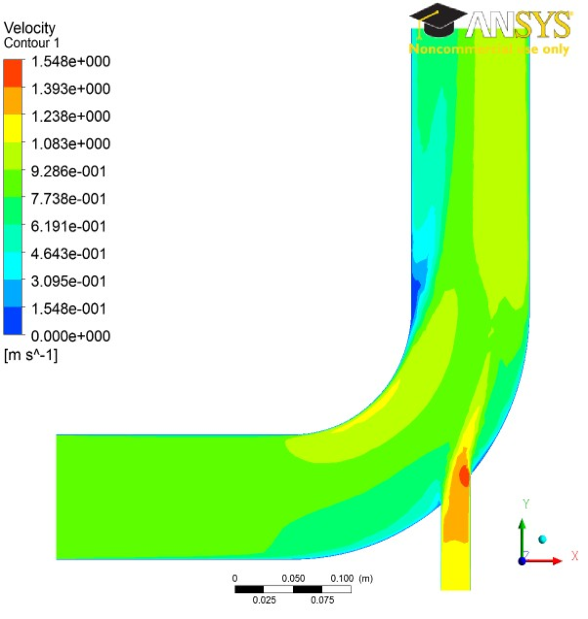
\includegraphics{background/5e1-1.pdf}
      \caption{Velocity distribution on the mid-plane for an inlet velocity for case 1.}
      \label{veldis}
\end{figure}
%%%%%%%%%%%%%%%%%%%%%%%%%%%%%%%%%%%%%%%%

The figure and caption should be centred. The figure numbering starts at 1 at the beginning of each chapter. The caption should provide a brief description of what is being shown. The figure should appear in the document after it is referred to in the text. No figure should be included which is not referred to in the text. Ensure that the size and resolution of images imported from software are sufficient to read any text.

\section{Tables}
Tables are an important way of displaying your results; Table \ref{tab:treatments} is a sample table, adapted from the Master/Doctoral Thesis template at \url{http://www.latextemplates.com/cat/theses}, which was generated with this code:

{\footnotesize
\begin{verbatim}
\begin{table}[b]
\caption{The effects of treatments X and Y on the four groups studied.}
\label{tab:treatments}
\centering
\begin{tabular}{l l l}
\toprule
\textbf{Groups} & \textbf{Treatment X} & \textbf{Treatment Y} \\\midrule
1 & 0.2 & 0.8\\
2 & 0.17 & 0.7\\
3 & 0.24 & 0.75\\
4 & 0.68 & 0.3\\
\bottomrule\\
\end{tabular}
\end{table}
\end{verbatim}
}

\begin{table}[b]
\caption{The effects of treatments X and Y on the four groups studied.}
\label{tab:treatments}
\centering
\begin{tabular}{l l l}
\toprule
\textbf{Groups} & \textbf{Treatment X} & \textbf{Treatment Y} \\
\midrule
1 & 0.2 & 0.8\\
2 & 0.17 & 0.7\\
3 & 0.24 & 0.75\\
4 & 0.68 & 0.3\\
\bottomrule\\
\end{tabular}
\end{table}

Tables are numbered in the same way as figures. Typically tables also have a short caption, but this is not universally true. The number and caption appear above the table, not below as with figures. Again, no table should appear in the report which has not been referred to in the text. Tables should come after they are discussed in the text. The exact formatting of the table depends somewhat on the content of the table, but in general, the text in the table should be the same font and size as the main text. 

\section{Equations}
All equations should be numbered sequentially. Do not restart the numbering at the beginning of each chapter. Unlike figures and tables, you may not need to refer to every equation in the text. You should take care to format equations properly. Do no simply try to use plain text. Use the equation layout facilities. An example of how equations should appear is shown in Equation \ref{sampleequation}. Here is the code for it:

{\footnotesize
\begin{verbatim}
\begin{equation}
\textrm{div}(\underline{u}) = \frac{\delta u}{\delta x} + \frac{\delta v}{\delta y} +
        \frac{\delta w}{\delta z} = 0
\label{sampleequation}
\end{equation} 
\end{verbatim}
}

\begin{equation}
\textrm{div}(\underline{u}) = \frac{\delta u}{\delta x} + \frac{\delta v}{\delta y} + \frac{\delta w}{\delta z} = 0
\label{sampleequation}
\end{equation} 

\section{Referencing published work}
It is important to give appropriate credit to other people for the work that they have shared through publications. In fact, you must sign a declaration in your report stating that you understand the nature of plagiarism. As well as avoiding plagiarism, citing results or data from the literature can strengthen your argument, provide a favourable comparison for your results, or even demonstrate how superior your work is.

There are many styles to reference published work. For example, the parenthetical style (which is also called the Harvard style) uses the author and date of publication (e.g. ``Smith and Jones, 2001''). There is also the Vancouver (or the citation sequence) style, which is shown in this document. In the Vancouver style, the publications are cited using a bracket number which refers to the list in the References section at the end of the report. The references are listed in order that they are cited in the report. A variant is name sequence style in which the publications are referenced by number, but the list is arranged alphabetically. For example, the text might say: several studies have examined the sound field around tandem cylinders generated by flow\cite{fitzpatrick2003flow,finnegan2010experimental}, while other investigations have focused on the effect of an applied sound field on the flow\cite{hall2003vortex}. Papers from conference proceedings\cite{jordan2001array}, books\cite{paidoussis2010fluid} and technical reports\cite{reyes2007power,iea2011} can be dealt with in the same style.

The Vancouver style has the advantage that it is a little more compact in the text and does not distract from the flow of the sentence if there are a lot of citations. However, it has the disadvantage that it is not immediately clear to the reader what particular work has been referenced.

It actually does not matter which particular referencing style is used as long as three important considerations are observed:
\begin{itemize}
\item the referencing style used throughout the document is consistent;
\item all material used or discussed in the text is properly cited;
\item nothing is included in the reference list that has not been cited.
\end{itemize}

This template has a suitable referencing style already set up -- you should use it and use the built-in BibTeX system to manage your references. See above for examples of how to cite a reference and look in the \texttt{sample.bib} file to see BibTeX references. Remember \href{http://scholar.google.com}{Google Scholar} and other search engines will give you BibTeX references for lots of academic publications. Otherwise, you can easily make up your own based on the examples in that file.
\chapter{Design}

\section{Introduction}
    The main objective of this project is to use existing automatic text summarisation methods to design a domain specific personalised summarisation system, that does not require use of superived domain specific models. The previous chapter’s review revealed methods, classifications and tasks of automatic text summarisation. This chapter describes the process of how the reviewed classifications, tasks, and methods were used to construct a summarisation system design that accomplishes the design objective of this project. A four step approach was taken in designing this system, seen in Figure \ref{design}. Step 1 of the design process was to determine the requirements of the design objective, to then define a classification of the required summarisation system. The definition created from this step both grounds the proposed system within the field of automatic text summarisation and limits the scope of methods that are to be considered in following steps of the design process. Step 2 of the design process was to identify the tasks to be performed by the summarisation system in order to fulfill the requirements of the design objective. The identified tasks describe the order of processes needed to be performed by the summarisation system. Identifying the system tasks provides an amature for which methods are applied, to construct a final system design. In Step 4, methods were examined and then selected to perform each of the identified system tasks based on their performance, satisfaction of system requirements, and compatibility with other methods selected for other tasks. The methods considered and then selected to perform the needed system tasks, were methods that fall under the same classification as the defined classification. With methods selected to perform summarisation tasks, an end to end personalised automatic text summarisation system was constructed that fulfills the requirements of the design objective. This chapter steps through the design process, presenting the design decisions made in developing the proposed system design.

\begin{figure}
    \centering
         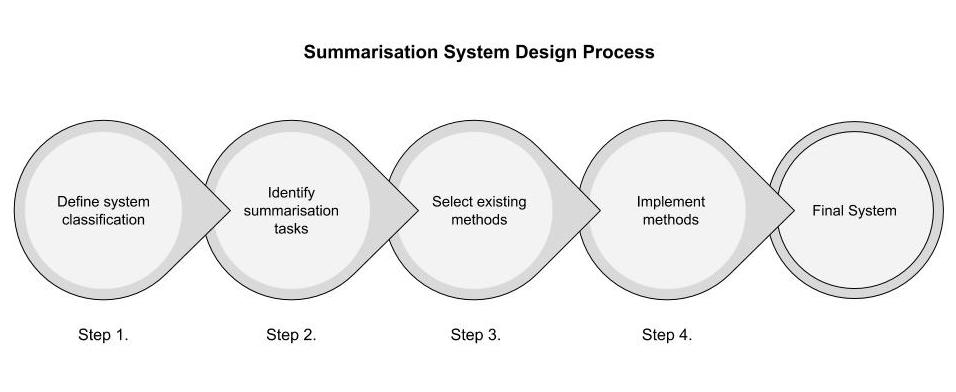
\includegraphics[width=1.0\textwidth]{Figures/Design_Process.jpg}
          \caption{Design process used for this project.}
           \label{design}
\end{figure}

\section{Requirements of The System}
To better describe the system, requirements are defined from the motivations and design objective of this project. The objective addressed in this chapter is to design a domain specific personalised summarisation system, independent of domain specific models from existing methods of extractive summarisation. The main motivation for such a system is to provide a summarisation on domains without formalised ontologies. The summarisation system purpose is to reduce information overload suffered by readers when reading multiple documents specific to a domain. From the motivation and design objective of this project the following requirements were defined for the needed summarisation system.

\textbf{R1:} The system operates on specific domain material without the use of formal supervised domain models.
\label{r1}

Summarisation systems are very good at reducing information overload as they maintain content across a set of documents while reducing the length and redundancy of which that content is discussed in the original documents. Domain specific summarisation systems produce better summaries from their comprehension of domain term relations and domain topic coherence. But these systems are often dependent on supervised models, which don’t exist for many domains of content on the internet. Thus this requirement aim is to produce a system design which performs domain specific summarisation within domains without formal ontologies. 

\textbf{R2:} The system forms summaries which significantly reduce the original content, while maintaining the most salient content, reducing the effects of information overload.
\label{r2}

Summaries best reduce information overload when they can minimise the content presented to the user without the loss of important content from the source documents. Thus in order for a system to reduce information overload it must attempt to reduce large amounts of textual content to its smallest, most salient form. Thus this specifies that this system must attempt to perform summarisation in a way that most greatly reduces original content inorder to have the best effect in reducing information overload.

\textbf{R3:} The system produces interpretable output that enhances user processing capabilities of the information being summarised.
\label{r3}

A user's ability to appropriately use a system often comes from their understanding of its operation. Providing interprobility of the system output helps a user understand why and how a summary is produced. Within a query-based system this can help a user adjust either the systems understanding or their query to better represent their information need, referred to as interactive information retrieval.  Including features of the original document from which the system used to construct a summary, allow for a summary not to act solely to inform a user but also to refer them to relevant documents which the content of the summary is presented in longer form. This is important because the usefulness of a summarisation is not solely limited to its summary readability and coverage of the source content.

\textbf{R4:} The system provides summaries which are personalised to a user's information needs.
\label{r4}
Personalisation is another method to further reduce the effect of information overload. Personalised summaries, also referred to as query-based summaries, require that the information summaries from a document set is specific to the information needed of the user. Performing a Personalised summarization is difficult within specific domains as the representation that is used must understand term relationships within a expressed query inorder to create a summary of relevant content. Thus this is required for the system as it must be able to understand term relations to allow for personalisation of summaries in a given domain.

\textbf{R5:} The system is constructed from existing extractive methods of summarisation that use topic representations as their immediate representation of source documents.
\label{r5}

Extractive methods don’t require semantic or natural language processing in the formation of the summary. Thus for the system to provide summarisation of unseen domains it must form summaries using extractive methods as they do not require supervised models for summary formation.

\textbf{R6:} The system is designed to be used with topic model based recommender systems.
\label{r6}

As discussed in the introduction one of the main motivations for this project is the similarity of constructing an extractive topic representation and automatically created ontologies, thus to serve this motivation the system should perform summarisation using a topic representation that is used in extractive summarisation. 

\section{Classifying the System}
This section presents the result of performing Step 1 of the design process. This step defines the system using a set of classifications derived from the system requirements. The classification of an automatic text summarisation system describes the system’s functionality at a high level. Preemptively defining the classification of a system, reduces the scope of methods and implementations to be considered for the inclusion in the system’s design, as well as providing a high level description of the system’s methods used to perform summarisation. In this section the classifications of automatic text summarisation are used to define the classifications of the required summarisation system. The selected classification for the system is shown in Figure \ref{fig:classification}. 

\begin{figure}[h]
    \centering
         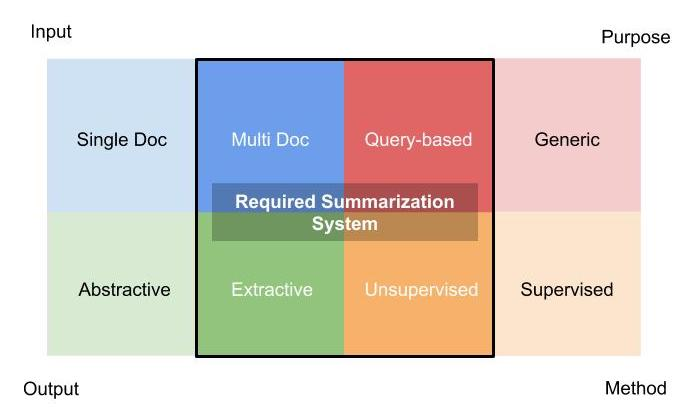
\includegraphics[width=.70\textwidth]{Figures/System_Classification.jpg}
          \caption{Classifications identified for the needed system.}
           \label{fig:classification}
\end{figure}

\subsubsection{Method: Unsupervised}
The most vital classification of the summarisation system is that the method of summarisation is unsupervised. As described by requirement \textbf{R1} of the system, the main motivation for this project is to provide a system which can provide domain specific personalised summaries without the need of supervised domain models. Such a system is required for the majority of content that exists without formal domain models. Domain ontologies are supervised even when automatically created. Inorder to design a system which is free from supervised domain models, the system must use unsupervised methods. Therefore the desired system can be classified as an unsupervised summarisation system.

\subsubsection{Input: Multi-Document}
Requirement \textbf{R2} of the system requires that textual content is reduced as much as possible to significantly reduce the effects of information overload. Summaries reduce information overload as they produce the most salient content from a document set. Inorder to best reduce the effects of information overload the summarisation the system must produce summaries from multiple documents. This also helps to satisfy requirement \textbf{R4}, as information related to a specified information need might be more likely to be spread across multiple documents then to be contained solely within a single document. Therefore the desired system can be classified as a multi-document summarisation system.

\subsubsection{Purpose: Query-based}
To satisfy requirement \textbf{R4} of the system design, the summaries produced by the system must be personalised. Personal summaries further reduce content presented to the user by considering their specific information needs. Personalised summaries are generated from an information need expressed as a query. Thus the desired system is classified as a query-based summarisation system. 

\subsubsection{Output: Extractive}
To allow for independence from formal ontologies the system must produce summaries that are created using extractive methods, satisfying requirement \textbf{R1} and \textbf{R5}. Abstractive summaries are reliant on domain semantic models, ontologies, or knowledge bases, thus extractive methods must be used so the system is independent of  supervised domain models. Extractive summarisation methods use topic representations, which are similar to ontologies. This similarity is one of the key motivations to the research question, and the system must be designed to be used with recommender systems, required in \textbf{R6}. Therefore the needed system is classified as an extractive summarisation system.

\subsection*{System Classification}
The classifications made for the summarisation system’s input, purpose, and output define the required domain independent personalised summarisation system as unsupervised, multi-document, query-based and extractive. This classification will be used by subsequent steps of the design process, to identify the necessary tasks and methods of the system.

\section{Identifying Summarisation Tasks}
This section presents the result of performing step 2 of the design process. Step of the design process identifies the tasks that the required system must perform. The tasks of a summarisation system are the operations that a summarisation system performs to produce a summary. While the tasks of a summarisation system do not directly describe the function of the summarisation systems, identifying the tasks required by a summarisation system provides an armature for which methods to perform tasks are applied.  The construction of methods from identified tasks presents the design of the summarisation system. This section identifies the tasks necessary for the system to perform to satisfy the requirements set from the design objective. The tasks identified for the required system were first derived from the universal set of tasks performed by all automatic text summarisation systems. From the universal tasks, accessory tasks were added that address the specific requirements of the desired system. The tasks identified in this section outline the operation of the proposed summarisation system in full.

As presented in Section \ref{sec:2.4} of the literature review, \citet{nenkova2012survey} define a set of tasks that are universal to extractive automatic summarisation systems. These universal tasks are:

\begin{itemize}
    \item Creation of an intermediate representation of documents.
    \item Scoring of sentences.
    \item Selection of setneces to form a summary.
\end{itemize}

From the foundation of these universal tasks, accessory tasks can be added that perform operations specific to the requirements of the summarisation system. The tasks identified for this system can be classified into tasks dependent on input document structure,  and tasks independent of docs. Both of these types of tasks exist within the system. To design a system which could be used with recommender systems (\textbf{R6}) external tasks that would be performed by a recommender system were also considered. The tasks identified are presented in Figure \ref{tasks}.

\begin{figure}[h]
    \centering
         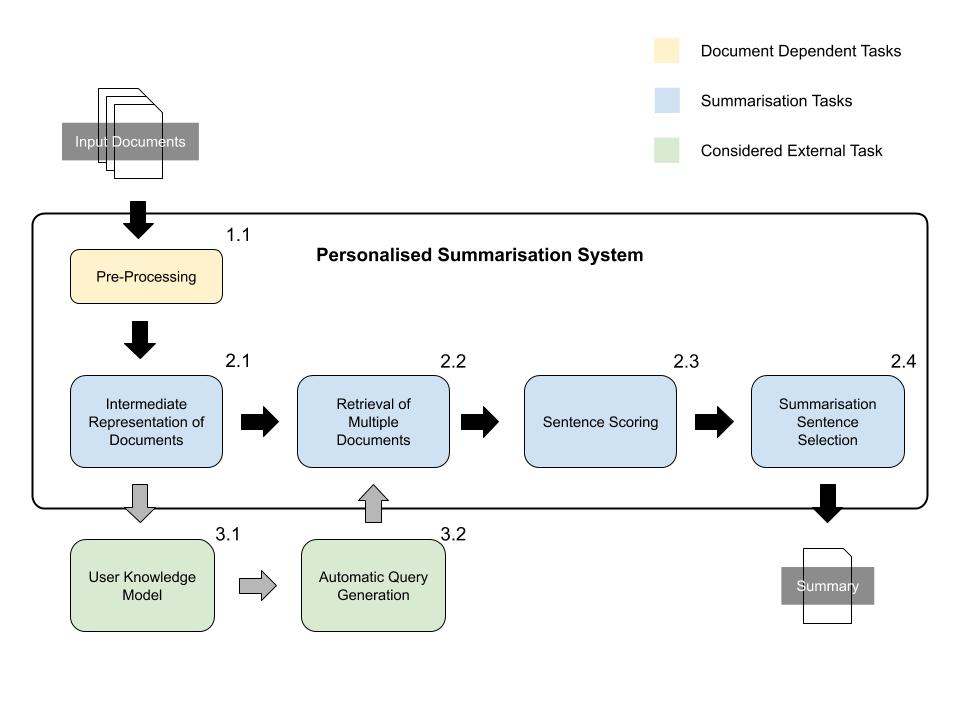
\includegraphics[width=1.0\textwidth]{Figures/Task_of_FYP_system.jpg}
          \caption{Tasks considered for the proposed system.}
           \label{tasks}
\end{figure}

\subsection{Task Group 1: Document Specific Tasks}
The tasks of this group are specific to the input documents. The aim of this task group is to prepare the raw input material to be used in the construction of the immediate representation, used in subsequent operations of the summarisation system. The method used to perform these tasks must directly address the features of the input documents, thus this task is classified as a document dependent task. In this system, the preprocessing 1.1 task is the only document specific task. Preprocessing refers to the operation of multiple methods that adjust the input material to be used in the creation of the immediate representation. Common operations performed by preprocessing tasks include: the removal of non-textual content, segmenting a document's textual content for the intermediate representation, as well as extraction of metadata from documents to be used in summary generation or in the output of the system. The method chosen to perform this task, would be altered if the type of input material was changed to a different form, such as news articles, academic journals, or social media posts. In this system the preprocessing task must address the specific operations necessary for xml structured Wikipedia articles used as input. The output from this task are textual elements extracted from the source material which allow for the intermediate representation 2.1 task to be performed.

\subsection{Task Group 2: Summarisation System Tasks}
The tasks of group 2 are tasks that are done by a summarisation system that are  independent of the source material. These tasks perform the core operations needed in producing summaries. From the classification and requirements outlined for the desired system, the operations carried out by this tasks group must serve the summarisation of multiple documents based on a personalised query. The tasks in this group have the following operations and output:

\textbf{Task 2.1}: This task creates an intermediate representation from the inputted pre processed documents. The intermediate representation of the text allows for the identification of salient sentences in the retrieval of documents task 2.2 and the scoring of sentences in task 2.3. The intermediate representation of documents has been specified by \textbf{R5} to be a topic representation, which aids in satisfying \textbf{R6} as topic representations are commonly used as well by the recommender system. Thus this task outputs representation of each document in the system as a set of topics.

\textbf{Task 2.2}: The retrieval of documents is an accessory task, not universally found in automatic text summarisation systems. The retrieval of documents task is specific to the system classification to produce query based summaries. This task uses a supplied query, from a recommender system or user, to select relevant documents. Because this system is classified as extractive, the summary is formed from document sets found relevant. Therefore the personalisation of the summary produced comes directly from the found relevant document set used in summary formation, aiding satisfying requirement \textbf{R4}. The output from this task is a subset of the input documents that have high relevance to the provided query.

\textbf{Task 2.3}: The sentence scoring task takes the sets of relevant documents and scores the sentences they contain based on the document topic representation given in task 2.1. The sentences with higher scores are those that cover the most salient material of the given document set, and thus should be prioritised for selection in the following sentence selection task. The output from this task is a set of scores from the sentences given from a set of relevant documents.

\textbf{Task 2.4}: In the summary sentence selection task 2.4 the inputted sentences and their scores are used to produce a summary of relevant material. Due to personalisation of content that is done in the document retrieval task 2.2, formation of this summary can be generalised to all the material it is given. The output from this task is a summary covering the most salient content from relevant material retrieved from task 2.2. 

\subsection{Task Group 3: External Recommender Systems Tasks}
Group 3 are tasks that are not part of the personalised summarisation system and thus were not included in the design or implementation of the system. These tasks are important to consider when selecting the methods to perform task 2.1 \& 2.2, as consideration for these tasks follows requirement \textbf{R6}, that the system should be designed to be used within a recommender system. Tasks of group 3 relate to the operations of recommender systems that would use the system's intermediate representation of documents to provide recommendations via queries. Recommender systems and user information need modeling is outside the scope of this project, but these tasks are to be considered so the summarisation system facilitates personalisation via a recommender system in possible future work.

\section{Selecting Existing Methods}
This section presents results of performing step 3 of the design process. This step produces a system design from the selection of methods to perform necessary operations of the required summarisation system, outlined by the tasks identified in Figure \ref{tasks}. The review of existing methods of extractive text summarisation in Chapter \ref{chp:2}, was used to inform the selection methods. Each task was approached by selecting a method from the existing summarisation systems. A method was selected to perform a task based on the following criteria:
\begin{itemize}
    \item The method performs well against other methods that perform the same task.
    \item The method helps satisfy one or more of the requirements outlined for this system.
    \item The method interfaces well with previously selected methods.
\end{itemize}

The methods that were examined and then selected for the system design, partially or completely fit under previously defined classifications of the system. It is important to note that the ordering in which methods are selected must respect dependencies between tasks. An example of task dependencies is the following, task 2.2 and task 2.3 are dependent on the intermediate representation method chosen for task 2.1, and the preprocessing done in task 1.1 is dependent on the intermediate representation task 2.1. The order that methods were selected for this system, respects these task dependencies. The selection of methods is presented chronologically in this section. From the selection of methods to perform a task, the methods which are selected on dependent tasks are further constrained, as they must interface with the method that was selected for a dependent task. From this process of selecting a method for each to perform the identified tasks, a design is presented which fulfills the requirements of the system thus satisfying the design objective of this project.

\subsection{Intermediate Representation}
The most important method to perform a task in the summarisation system is the method used to intermediately represent documents. This task's importance comes from the dependency of other methods that are used for the tasks of preprocessing, retrieval, and scoring are reliant on the method chosen to form the intermediate representation of documents. The methods examined to possibly perform the formation of intermediate representation were extractive summarisation methods that use topic representations, reviewed in Section \ref{subsec:2.3.1}. Extractive topic representation methods satisfy the requirement that the system is extractive as well as the requirement that the system design can be used with topic model based recommender systems. The method selected to intermediate represent documents for this system is topic model formed from the Latent Direlect Allocation (LDA) method.

\subsubsection{Latent Direllect Allocation Topic Representation}
\label{subsec:3.5.1}
Latent Direllect Allocation is an unsupervised generative probabilistic method for modeling a corpus (i.e. document set). LDA represents each document in a corpus as a probabilistic distribution over a number of latent topics. Every latent topic is made up of a probabilistic distribution over all words in the corpus. The mathematical representation of this method is as follows:

A given corpus $D$ consists of $M$ documents, document $d$ having $N_d$ words.
The model is formed from the following generative process
\begin{enumerate}[(a)]
      \item Choose a multinomial distribution $\phi_t$ for topic $t$ ($t \in \{1,\dots,T\}$) from a Dirichlet distribution with parameter $\beta$.
      \item Choose a multinomial distribution $\theta_d$ for document $d$ ($d \in \{1,\dots,M\}$) from a Dirichlet distribution with parameter $\alpha$.
      \item For a word $w_n$ ($n \in \{1,\dots,{N_d}\}$) in document $d$.
      \begin{enumerate}
            \item Select a topic $z_n$ from $\theta_d$.
            \item Select a word $w_n$ from $\phi_{zn}$
      \end{enumerate}
\end{enumerate}
In this process the words in documents are the only observed variable, while other variables are latent ($\phi$ and $\theta$) and hyper parameters ($\alpha$ and $\beta$). To infer the latent variables and hyper parameters, the probability of observed data $D$ is maxmised by (\ref{ldaUpdate}).

When an unseen or seen document is given to the model the output is a probabilistic distribution of latent topics. These probabilistic distributions can be used with metrics such as cosine similarity to determine the similarity of documents for retrieval. The formation of LDA topic models is done solely on a corpus of documents, satisfying the requirement of the system of being independent of domain specific models, \textbf{R1}. Extractive summarization methods that use LDA models for topic representations have also shown good performance for multi-document summarisation \citep{daume2006domain,wang2009multi}. When the set of documents used to create the model is a corpus of domain documents, LDA’s topic model is a representation of the term to topic relations of that domain. LDA topic models are also commonly used in user modeling in recommender systems \citep{pandit2013query, harvey2013building, mehrotra2015terms}. This common model for document representation and user understanding could be used in extending the system to perform summarisation as part of a recommendation system. LDA compared to other methods had strong performance, and satisfaction of requirements \textbf{R1, R5,} and \textbf{R6}. With LDA used as the intermediate topic representation of documents, methods for performing preprocessing, document retrieval and sentence scoring were further constrained to methods that work with a LDA intermediate representation.

\subsection{Preprocessing}
\label{subsec:3.5.2}
Preprocessing refers to the extraction of textual content from a corpus of raw documents. The textual content extracted from source documents is used by a subsequent method to create an intermediate representation. The method chosen to perform preprocessing for this system, must respect both the structure of the source content (Wikipedia articles) as well as produce an output in the form needed by the intermediate representation method, LDA. To respect the structure of input documents, methods of preprocessing were selected from existing systems that operate on news articles. Both news articles and historical Wikipedia articles are based on a singular subject and present events and explanations based on the article’s subject matter. Thus the preprocessing for news articles and historical Wikipedia articles can be assumed to be similar, based on the similarity of their content.  To produce preprocessed text in a form that respects the LDA method for performing intermediate representation, methods of preprocessing were selected from summarisation systems that also use LDA for their intermediate representation. Combining methods of preprocessing from similar systems produces a method of preprocessing for this system that respects both the input documents and the intermediate representation of this system.

\subsubsection{Text Normalisation}
Natural text is presented in a form that is readable to humans. Text normalisation is the process of transforming natural text to a form that is more readable to a machine. Text normalisation is a common task in natural language processing. Text normalisation cleans the raw natural text to be better used in creation of a LDA topic representation of a document's content. Text normalisation methods to be used for LDA are the conversion of all words to lowercase, removing punctuation, removing of stopwords, expanding abbreviations, and canonicalization of words. These steps are standard and are produced by most systems that use LDA.

\subsubsection{Article Representation}
Identifying the structure of the input documents helps to determine how textual content should be inputted into the method used for the intermediate representation. In this project the input documents to be used for summarisation are 32 Wikipedia articles related to the Watergate Scandal. Wikipedia articles use an encyclopedic style to present information relating to a specific topic. Wikipedia articles present information in a structure where each paragraph discusses a topic in a specific context. It is important to note that LDA has been shown to have better accuracy when performed on a large corpus set \citep{crossley2017important}. The corpus used for this system is relatively small. In an attempt to increase accuracy and to construct a model that is representative of the paragraph styling of Wikipedia articles, each paragraph in an article was treated as a separate document. This hopes to improve performance that would otherwise be suffered from treating each article as a separate document. Metadata from a document source article, such as the title and url, is also maintained to be used in explanation of the system generated summary. This helps with satisfying requirement \textbf{R3} of the system, by enhancing user processing of summary information via references to the articles from which the extractive summary was formed from.

\subsubsection{Concept Extraction}
Extractive summarisation systems that process similar documents to the Wikipedia article for use in a LDA topic representation were examined to select a method to perform preprocessing for this system. The original implementation of LDA uses a bag-of-words representation to create a topic model \citep{blei2003latent}. Recent work on news article summarisation systems that use LDA, have found better summarisation performance by using a bag-of-concepts representation of document content \citep{rajagopal2013commonsense,li2016cross,raviv2016document}. A bag-of-words representation treats each document as a list of sentences, where each sentence is a list of words contained in the corresponding sentence. A bag-of-concepts changes out the sentence list to contain concepts of a sentence rather than words. For each sentence a list of concepts is created. A Part of Speech Tagger is used to tag words with their parts of speech (POS) in each sentence. Word pairs are extracted from a tagged sentence by selecting specific POS, such as verb noun pairs, nouns, and named entities. The word pairs are then normalised into concepts by centralising terms into common meaning, via a semantic model. These normalised word pairs are the concepts that make up a list which sentence is represented by. For example the sentence “Vice President Gerald Ford succeeded to the presidency upon Nixon's resignation.” is represented in the POS dependency tree in Figure \ref{pos}. 

\begin{figure}[h]
    \centering
         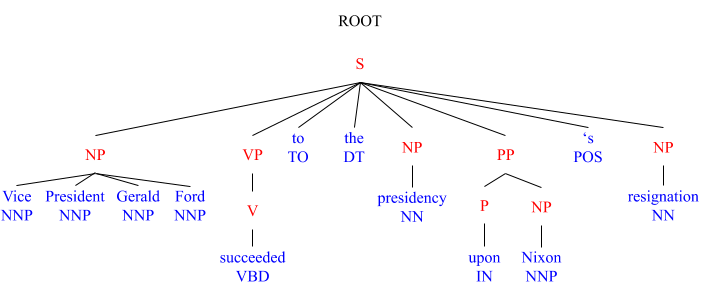
\includegraphics[width=1.0\textwidth]{Figures/POS_TREE.png}
          \caption{POS dependency tree for "Vice President Gerald Ford succeeded to the presidency upon Nixon's resignation".}
           \label{pos}
\end{figure}

The dependency tree is traversed to extract necessary POS to represent concepts. An example of this is the extraction of such as a noun pair (NP), n-gram pairs of nouns referring to a single object. The extracted noun pairs from this example would be: “Vice President Geral Ford”, “presidency”, “nixon” and “resignation”.

The bag-of-concept representation achieves better performance than the traditional bag-of-words representation. The performance of the LDA is increased by reducing the noise in the LDA topic model that occurs when unimportant words from the text are used in the topic word distributions. The bag-of-words representation treats all words as independent, disregarding dependencies between words. The bag-of-concept representation attempts to respect the dependence of words, resulting in an improvement in the accuracy of the model in representing the source content, as well as limiting noise by only including the most representative word grouping of a sentence’s meaning.

The method chosen for this system is a stripped down approach to other bag-of-concept document representation implementations. The stripped down approach was taken to avoid the use of semantic models to normalise extracted concepts. The method selected for the system extracts just noun pairs and named entities. A semantic model is not used to centralise concepts. The method therefore treats the extracted concepts: “president nixon”, “richard nixon” and “nixon” independently. This simpler approach was done in an attempt to build the summarisation system with no reliance on semantic models, satisfying requirement \textbf{R1}. Without centralising concepts the LDA model accuracy is expected to be reduced compared to a model built with normalised concepts, but this method should provide better performance compared to traditional bag-of-concept methods of preprocessing. 

\subsection{Document Retrieval}
\label{subsec:3.5.3}
The method selected to perform the retrieval of multiple documents utilizes the intermediate representation of all documents to produce a subset of documents that are relevant to a given query. The set of relevant documents is used for the scoring and summarisation tasks of the system to produce an extractive summary. The system’s ability to personalise summaries comes from how well the system can determine a users information need from a query and how well the system is able to find documents that satisfy that information need. To address these factors document retrieval was broken up into two processes. The first process is a method for which a given query is expanded. Query expansion is a common method performed in information retrieval. Query expansion reduces the number documents found relevant from adding terms to the query. Additional terms further specify information needed for the query making it more specific. The second process is the method in which a query is used to retrieve relevant documents. Together these processes form the method used for retrieving documents relevant to a query.

\subsubsection{Process 1: Query Expansion}
Query expansion is a common information retrieval task. Queries are expanded by taking an original query and adding content to it based on the system's interpretation of the queries meaning. Expansion increases the performance of document retrieval by limiting document and query mismatching \citep{carpineto2012survey}. Due to this being reliant on the systems interpretation of document content, methods that attempt to expand queries using a LDA topic model presentation were examined. 

The method chosen for performing query expansion is proposed by Li and Jin’s \citeyear{li2016cross} paper “Cross-document knowledge discovery using semantic concept topic model.” In \emph{2016 15th IEEE International Conference on Machine Learning and Applications (ICMLA)}. The method they present forms concept chain queries, which attempt to detect links between two topics of interests across documents. Given a query that contains concept A and concept C, this method uses the topic representation to determine the path between concept A and C, expanding the query with the inclusion of intermediate terms of concept B. The algorithm for the method is as follows:

\begin{enumerate}
    \item Conduct an independent search for concept A and concept C, and collect relevant sentences in which A and C appears. These sentence sets are defined as AS and CS;
    \item Union set AS and CS to form a new document collection. This new set is the relevant context for the query pair A and C and is used in the subsequent topic discovery sent, this set is referred to as BS;
    \item Apply LDA model on BS and generate topically relevant terms for A and C. The generated terms are constrained to concepts appearing in the original dictionary of the LDA model;
    \item For each topic determined by the model on set BS identify top semantic concepts, which serve as B level terms connect A and C topically;
\end{enumerate}

A query given by a user might contain two domain terms that are not closely related. With systems that use domain models this is easily handled, as ontologies or semantic models can be traversed to find a common parent concept or term. The method selected for query expansion emulates an ontology based approach by smoothing conceptual jumps by adding terms that have common relationships to the domain concepts presented in the original query. Since the system produces an extractive summary directly from the documents relevant to a query, the expanded query from this method should produce documents that link logical jumps in the original query, producing a summary that is able to connect logical jumps of domain specific terms. 

\subsubsection{Process 2: Query-Based Retrieval}
The goal of query based document retrieval is to produce a set of relevant documents based on a given query. This is approached by scoring all documents for their relevance to a given query and then selecting the n-most relevant documents as an answer. The scoring for relevance has many approaches, and is its own field within computer science. Many methods exist that use LDA query based document retrieval. The LDA topic model can produce a topic distribution for an unseen document. Thus LDA can be used for assessing the topic distribution of a given query and then determining documents that are relevant to that topic distribution. The output from passing a query to the LDA model is the probability of topics that query relates to based on the words that a query contains. With the same topic distribution given for documents the probability of producing a given query given a document can be determined. Documents that produce higher probabilities of producing the given query are then treated as more relevant. Methods that directly use the LDA topic model probabilities, heavily rely on the accuracy of the topic model. Due to the small corpus size used in designing this system, the LDA topic model formed from the corpus is more susceptible to inaccuracy \citep{crossley2017important}. Other LDA based approaches for retrieval use the topic distribution of documents and query to calculate similarity. Highly similar documents to query are then treated as relevant \citep{steyvers2007probabilistic}. These methods are not as direct as using direct probabilities, and therefore are less reliant on the accuracy of the model. Therefore The method chosen for retrieval in this system is the cosine similarity of a document topic distribution and a query distribution.

When a query is given to the system, all of the documents are scored based on the cosine similarity \ref{cosim} of the document’s topic distribution at the topic distribution of the query. When a document, a wikipedia article or user query, is input into the LDA model, a vector of topic ids and corresponding weights are given. Cosine similarity can be calculated as follows:

Consider the two topic distributions $\vec{Q}$ for query and $\vec{D}$ for document. Each contains $k$ probabilities of them relating to each of the $k$ topics in the topic model. The similarity of the distributions can be calculated by:
\begin{equation}
    cossim(\vec{Q}, \vec{D}) = \frac{\sum_{i=0}^k q_i \times d_i}{\sqrt{\sum_{i=0}^k q_i^2}\sqrt{\sum_{i=0}^k d_i^2}}
    \label{cosim}
\end{equation}
All documents are scored against a query and the documents selected to be relevant are those with a similarity above a specified threshold. LDA is not the best used method for document retrieval. \citet{wei2006lda} present that LDA itself is too coarse of a representation to be used as the sole representation for document retrieval. Considering this is a component of a larger system using the LDA topic model for retrieval is sufficient, as it interfaces well with the existing LDA topic representation of the system.

\subsubsection{Document Retrivel Method: Process 1 \& 2}
The method used for the retrieval of multiple documents from a query is as follows. For each imputed query, it is expanded with terms that relate to its topic representation, then all documents are scored based on their cosine similarity with the expanded query. Documents are returned if their similarity is above a threshold. This method results in a document set to be used in the formation of a summary. The summary is personalised from the query relevant content found relevant based by this method. 

\subsection{Sentence Scoring and Summary Selection}
label{subsec:3.5.4}
Sentence scoring is used in the selection of document sentences for a summary. The aim of sentence scoring in extractive summarisation is to score sentences in respect how well they cover the content of the documents being summarised. These scored sentences are then used in a method which selects  sentences based on their scores to form a summary. For both these tasks are implemented via a method that includes the scoring and selecting of sentences as one. The method chosen for sentence scoring as well as sentence selection is the method presented by Alguliev et al. \citeyear{alguliev2011mcmr} “MCMR: Maximum coverage and minimum redundant text summarization model” in \emph{Expert Systems with Applications}. The method presented by Alguliev et al, outperforms other methods of performing extractive summarisation \citep{gambhir2017recent}. This method is also unsupervised and requires no other representation or pre processing of textual content. Thus this method was easily identifiable as the method to perform sentence scoring and summary generation for the required system.

\subsubsection{Sentence Selection}
Considering a document collection $D = \{d_1,d_2,\dots, d_{|D|}\}$ where $|D|$ is the number of documents. Each document contains a set of sentences $d_i = \{s_1,s_2,\dots,s_{|d_i|}\}$ where $|d_i|$ is the number of sentences in the ith document. This method considers the document collection as a set of all sentences $D = \{s_1,s_2,\dots,s_n\}$ where $s_i$ is the ith sentence in document collection $D$ and $n$ is number of sentences in the document collection. $T = \{t_1,t_2,\dots,t_m\}$ represents all the terms occurring in $D$, where $m$ is the number of different terms. The method attempts to find the subset of the sentences  $D = \{s_1,s_2,\dots,s_n\}$ that covers the main content in the document collection. $S$ be the set of sentences constituting a summary, the similarity between the document collection and the summary is $sim(D,S)$, which is what is going to be maximised. The length of a desired summary is used as a cardinality constraint on the maximisation of $sim(D,S)$, so that summary is of length $L$ or shorter, where $L$ is a number of words in the summary. This formalises the summarsation problem as follows:
\begin{equation}
    Maximise \; sim(D,S) \\
    s.t. \; len(S) \leq L
    \label{mcmrSimple}
\end{equation}

This alone does not minimise the redundancy in the produced summary. Thus the following formalisation is used. 

Let $x_{ij}$ denote a variable which is 1 if the pair of sentence $s_i$ and $s_j$ are selected to be in the summary, otherwise 0, and $len(s_i)$ denote the length of sentence $s_i$. Thus assuming that each sentence is a candidate summary sentence the problem can be written as:
\begin{equation}
    Maximise \: f = \sum_{i=1}^{n-1} \sum_{j=i+1}^n [sim(\vec{D}, \vec{s_i}) + sim(\vec{D}, \vec{s_j}) - sim(\vec{s_i}, \vec{s_j})]x_{ij}
    \label{mcmrGeneral}
\end{equation}
\begin{equation}
    s.t. \; \sum_{i=1}^{n-1} \sum_{j=i+1}^n [len(s_i) + len(s_j)]x_{ij} \leq L
    \label{mcmrConstraint}
\end{equation}
\begin{equation}
    x_{ij} \in \{0,1\} \forall i,j
    \label{mcmrVar}
\end{equation}

Now the objective is to find the binary assignment on $x_{ij}$ with the highest score,best coverage and least redundancy, such that summary length is at most $L$. This formation is an integer linear programming problem where both the object function and constrained at the linear set of integer variables. The object function guarantees that the produced summary will be covered by the summary from the first and second terms in \ref{mcmrGeneral}. The third term also guarantees that the summary will not contain multiple sentences that convey the same information, reducing redundancy. The integrality constraint on $x_{ij}$ is automatically satisfied in \ref{mcmrVar}.

\subsubsection{Sentence Scoring}
This system uses two scores for sentences and the score of a sentence is a weighted sum based on a specified alpha value. The two scoring metrics are a cosine similarity of TF-ISF (Term Frequency, Inverse Sentence Frequency) scores of terms in a sentences and the Normalised Google Distance. 

\textbf{Cosine Similarity of TF-ISF}
Each sentence is represented as a vector of weighted terms given by their TF-ISF scores. $s_i =\{w_{i1};w_{i2}; \dots; w_{im}\}$ where $m$ is the number of terms in the document collection, $w_{ik}$ is the weight of term $t_k$ in the sentence $s_i$. The element $w_{ik}$ is defined using the TF-ISF, given in \ref{tfisf}.
\begin{equation}
    w_{ik} = f_k \times \log(\frac{n}{n_k})
    \label{tfisf}
\end{equation}
Where $f_k$ is the term frequency the number of occurence of term $t_k$ in sentence $s_i$, $n_k$ denotes the number of sentences in which $t_k$ appears and $n$ is the number of sentences. The $\log(\frac{n}{n_k})$ is referred to as the isf factor. TF-ISF assigns a weight to term $t_k$ in a sentence $s_i$ that is:
\begin{enumerate}
    \item Highest when $t_k$ occurs many times in a small number of sentences;
    \item Lower when a term occurs few times in a sentence, or occurs in many sentences;
    \item Lowest when the term occurs in virtually all sentences;
\end{enumerate}

From the vectors of weights for each term in two sentence, $\vec{s_i}$ $\vec{s_j}$, the cosine similarity is calculated.
\begin{equation}
    sim_{cos}(\vec{s_i},\vec{s_j}) = \frac{\sum_{k=1}^m w_{ik} w_{jk}}{\sqrt{\sum_{k=1}^m w_{ik}^2}\times\sqrt{\sum_{k=1}^m w_{jk}^2}}, i,j=1,\dots,n
    \label{cossimSent}
\end{equation}


\textbf{NGD-Based Similiary}
To calculate normalised google distance similarity each of sentence is represented by a list of terms. $s_i=\{t_1,t_2, \dots, t_{|s_i|}\}$ where $|s_i|$ is the number of distinct terms in sentence $s_i$. The similarity of sentences $s_i$ and $s_j$ can be calculated using:
\begin{equation}
    sim_{NGD}(s_i, s_j) = \frac{\sum_{t_k \in s_i} \sum_{t_l \in s_j} sim_{NGD}(t_k,t_l)}{|s_i| \times |s_j|}, \\ where \; sim_{NGD}(t_k,t_l) = \exp(-NGD(t_k, t_l))
    \label{ngdSent}
\end{equation}

\begin{equation}
    NGD(t_k,t_l) = \frac{max\{\log(f_k), \log(f_l)\}-\log(f_{kl})}{\log n - min \{\log(f_k),\log(f_l)\}}
    \label{ngdTerm}
\end{equation}
Where $f_k$ is the number of sentences term, $t_k$ appears in, $f_kl$ is the number of sentences both $t_k$ and $t_l$ appear in, and $n$ is the number of sentences in the document collection.

These similarity measures are both used making the true formula for MCMR summary formation the following.
\begin{equation}
    Maximise \: f_{\alpha} = \alpha \times f_{cos} + (1-\alpha) \times f_{NGD},
    \label{mcmrFull}
\end{equation}
$where$
\begin{equation}
    f_{cos} = \sum_{i=1}^{n-1} \sum_{j=i+1}^n [sim_{cos}(\vec{D}, \vec{s_i}) + sim_{cos}(\vec{D}, \vec{s_j}) - sim_{cos}(\vec{s_i}, \vec{s_j})]x_{ij}
\end{equation}
\begin{equation}
    f_{NGD} = \sum_{i=1}^{n-1} \sum_{j=i+1}^n [sim_{NGD}(\vec{D}, \vec{s_i}) + sim_{NGD}(\vec{D}, \vec{s_j}) - sim_{NGD}(\vec{s_i}, \vec{s_j})]x_{ij}
\end{equation}

\subsection{System Design with Methods}
With the methods selected to perform each of the identified tasks, the design in Figure \ref{designD} is constructed. The design represents four main processes of the system, each of which are  performed from the selected methods of this section. This design can also then be compared directly to the original requirements outlined for the system, to determine if it achieves the requirements necessary to achieve the design objective of this project.

\begin{figure}[h]
    \centering
         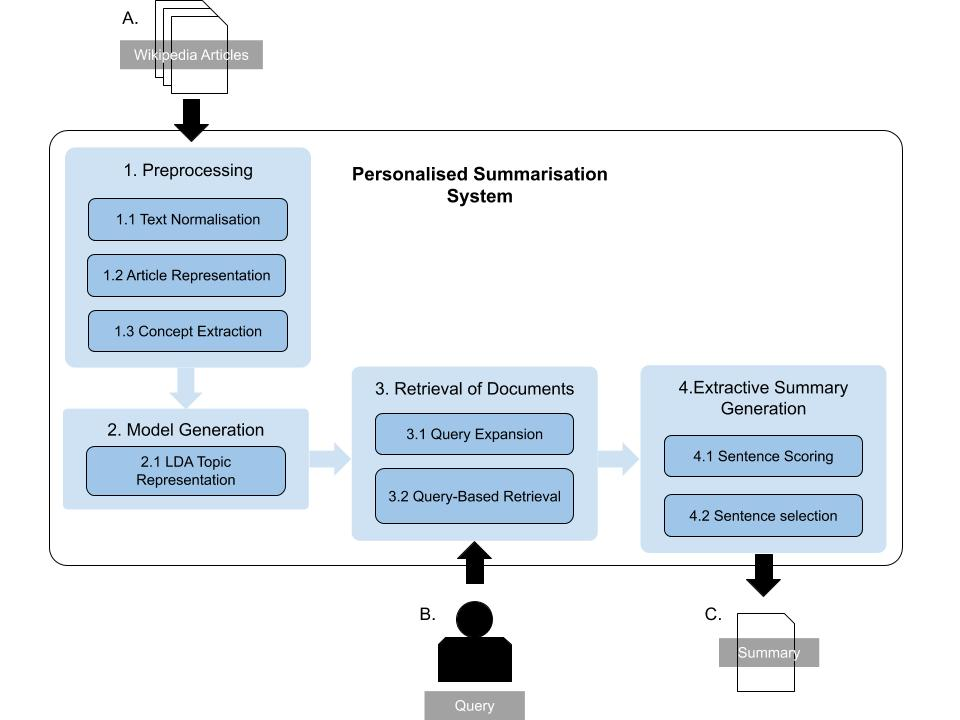
\includegraphics[width=0.80\textwidth]{Figures/System_Design_from_Design_Chapter.jpg}
          \caption{Design developed from the classification, tasks, and methods identified for the needed system.}
           \label{designD}
\end{figure}

The four processes in the system design are Preprocessing, Model Generation, Retrieval of Documents, and Extractive Summary Generation. These processes are constructed from the methods selected to perform the identified tasks needed by the system. Together their functionality explains the functionality of the proposed Personalised Summarisation System. Preprocessing includes the methods used for identified tasks of preprocessing. These methods include text normalization, article representation and concept extraction. From the Preprocessing process a bag-of-concepts representation is constructed from the raw Wikipedia article input. The bag-of-concepts is used in the Model generation process which uses the LDA method to create a topic model of all content in a domain. This topic model is used in the Retrieval of Documents, to expand a given query and then assess document similarity from the domain set of documents to produce a set of relevant domain documents related to a query. The set of relevant documents is then used in the Extractive Summary Generation Process. Here the sentence scoring and sentence selection methods find the most salient sentences from the retrieved documents and extractive summary is produced. The design addresses and satisfies all of the requirements outlined for the needed system.

\textbf{R1:} The system operates on specific domain material without the use of formal supervised domain models.

The design uses no supervised models for either the modeling of a domain or in producing a summary. Certain methods, such as concept extraction, were modified from their original implementations to be independent of supervised models. The LDA topic representation can model a domain when given a complete set of documents that describe the domain providing system understanding of domain terms and their relationships as topics. Lastly the use of query expansion can smooth domain topic jumps that exist within a query, achieving similar functionality to supervised domain models, while being unsupervised. Thus the system here is designed to operate on domain material without the used of supervised models.

\textbf{R2:} The system forms summaries which significantly reduce the original content, while maintaining the most salient content, reducing the effects of information overload.

The personalised retrieval of documents used in forming an extractive summary greatly reduces the effects of information overload, by not only limiting information presented  to a user to be most relevant to their information need, but by also producing a summary which presents the most salient content of those retrieved documents in a short digestible form. Thus this system takes a two fold approach to limiting information overload, by reducing content to a small set of most relevant documents to a query and then producing a summary from the relevant document that maximises its coverage of material in the relevant document. This approach significantly reduces the effects of information overload, and thus satisfies this requirement.

\textbf{R3:} The system produces interpretable output that enhances user processing capabilities of the information being summarised.

In the Preprocessing process, all sentences to document and document to article relationships are maintained. With the summary these relationships can be given to a user to provide the articles in which sentences originated from in the summary. Other components lend themselves to providing interpretable output, such as the expanded query created in the document retrieval process. The expanded query identifies additional concepts which are related to concepts in the query, giving the user an understanding of the system’s interpretation of their query. The user can then adjust their query based on the system's presented interpretation allowing for the user to adjust their query to better address the true information need known as interactive information retrieval. The system methods allow for additional output to be provided which help give interpretability to an end user. 

\textbf{R4:} The system provides summaries which are personalised to a user's information needs.

The design provides personalised summaries, from producing summaries from a document set that are relevant to a given query. A given query specifies an information need, which the system satisfies by providing relevant documents from the corpus that are similar to the expressed information needed. These documents are then used in the formation of an extractive summary. Because the summary is produced from a personalised set of relevant documents itself is thus personalised to the information needed in a query.

\textbf{R5:} The system is constructed from existing extractive methods of summarisation.

Every method contained in this design was selected from systems or methods that were classified as extractive. So not only does the method for producing a summary produce them  extractively, it is supported by other methods that enhance the extractive summary formation. 

\textbf{R6:} The system is designed to be used with topic model based recommender systems.

The system uses a LDA topic representation. This representation is also commonly used by the recommender systems, to model user knowledge or interest. Thus a recommender system could share the intermediate representation of documents to produce information needs as queries. Thus the system is easily housed within a recommender system.

This design satisfies the requirements presented at the beginning of this chapter, thus satisfying the design objective of this project. Through implementation of this design the system can be assessed to determine the extent that existing automatic extractive summarization methods can be used to provide domain specific personalised summaries, independent of domain specific ontologies and semantic models.

\section{Summary of Design}
This section presented the process in which the review of automatic text summarisation literature was used to construct a domain specific personalised summarisation system, that does not require use of superived domain specific models. First a set of requirements for the system were outlined using the design objective and motivations of the project. Then the first 3 steps of the 4 step design process were completed to produce a system design that satisfies the outlined requirements, therefore producing a system that satisfies the design objective of the project.  First the classification of the system was defined. This provided a description of the  system’s functionality at a high level and grounded it within the field of automatic text summarisation. The classification of the system was then used to identify tasks to be performed by the summarisation system, identified from systems with similar classifications. Then methods were selected based on its performance, satisfaction of requirements, and compatibility with other selected methods for system tasks. With all methods selected a system design was constructed which was assessed against the requirements set at the beginning of this chapter. The design satisfied all of the requirements set and thus the presented design satisfies the design objective of this project of using existing automatic text summarisation methods to design a domain specific personalised summarisation system, that does not require use of superived domain specific models. The design produced in this chapter is used in the following chapter to implement this system, to then assess the proposed system in regard to this project's research question.
\chapter{Implementation}
This chapter presents the implementation of the design of the proposed summarisation system. The implementation presented in this chapter was used to assess the design’s limitations and efficacy for performing domain specific personalisation without the use of domain models. The methods used in the system design were implemented from their respective papers. Due to the availability of libraries available for text processing and topic modeling, this system was implemented using python 3.7.4 \citep{van2009python}. The existing methods selected to perform tasks of the system were implemented within python classes. Each python class encapsulates a number of methods from the identified design. The class structure for which the methods were implemented is unimportant to the system’s functionality, so this chapter will focus on the operations performed, using these classes. The functionality of the implemented system is presented in Figure \ref{designI}. The system uses three main processes to create extractive personalised summaries. Each process contains a set of relevant child processes. First, the Model and Corpus Generation process creates an annotated corpus and a topic model from a set of raw Wikipedia articles. Then the Query-based Document Retrieval process uses a query to retrieve relevant documents using the annotated corpus and topic model. Last, the Summary Generation process creates a summary from the sentences contained within the query relevant documents. Each of these processes implementations is presented in detail in sections of this chapter. 

\begin{figure}[h]
    \centering
         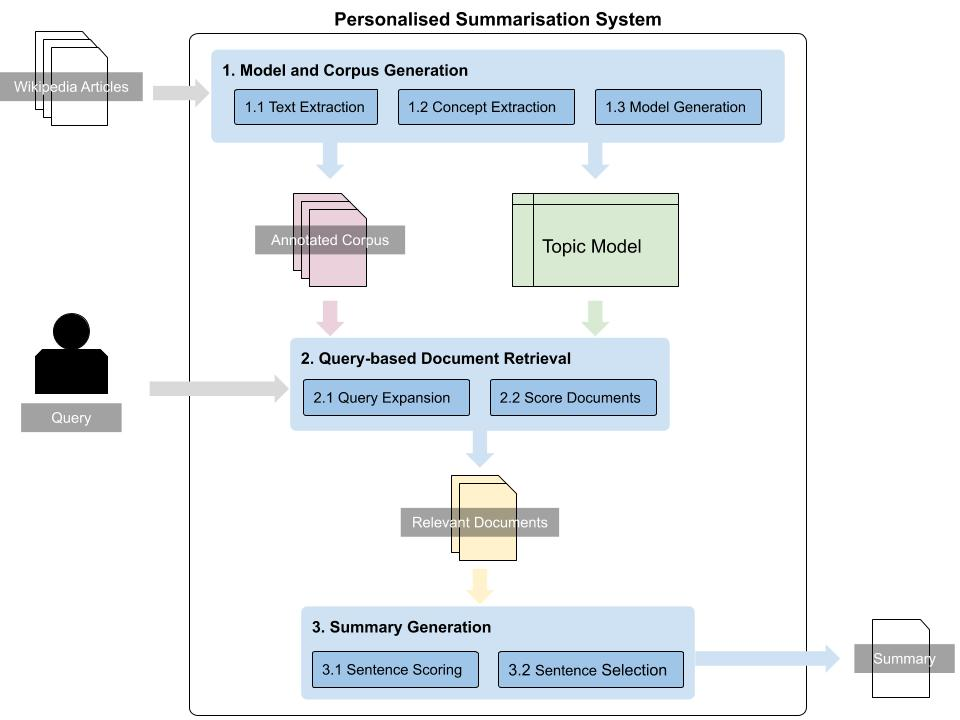
\includegraphics[width=0.70\textwidth]{Figures/System_Design_Overview.jpg}
          \caption{Design of system implemenation processes.}
           \label{designI}
\end{figure}

\section{Model and Corpus Generation}
The Model and Corpus Generation process of the system produces a meta-data annotated corpus and topic model. This process of the system is done via three child processes, text extraction from source material, concept extraction from text, and the creation of an annotated corpus used in the creation of a topic model. These processes are broken down in Figure \ref{modelDesign}.

\begin{figure}[h]
    \centering
         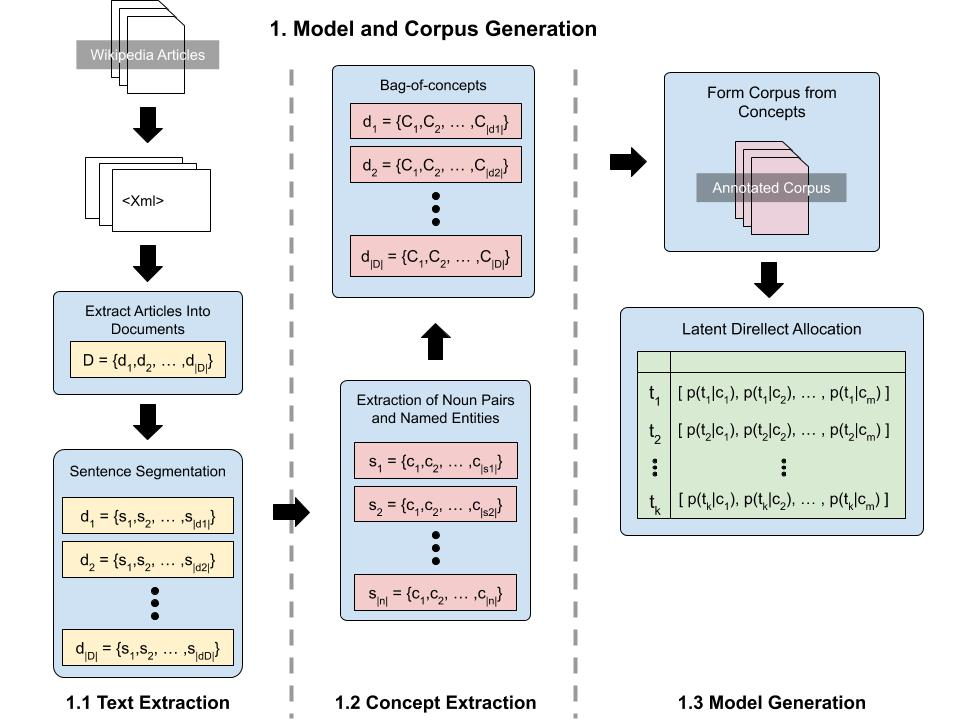
\includegraphics[width=0.70\textwidth]{Figures/System_Design_Model_Gen.jpg}
          \caption{Process of Model and Corpus Generation.}
           \label{modelDesign}
\end{figure}
Where $D$ is the document set extracted from articles, and $|D|$ is the number of documents extracted from source articles. $s_i$ is sentences in each document and $|d_i|$ is the number of sentences in each document. $c_i$ are the concepts extracted from $s_i$ and $|s_i|$ is the number of concepts in sentence $s_i$. $C_i$ is the set of concepts in sentence $s_i$. $t_i$ are the latent of topics determined by the model given $k$ is the number of topics. $m$ is the number of different concepts found in corpus $D$.

\subsection{Text Extraction}
This process takes a set of Wikipedia articles and extracts their textual content to be used in the creation of the corpus which is used in the formation of the topic model. Articles were downloaded using Wikipedia’s export system\footnote{\url{https://en.wikipedia.org/wiki/Special:Export}}. The export consists of a XML document that contains articles based on a given list of article titles. The list of articles were those that were in the category of “Watergate Scandal” on Wikipedia. The Wikipedia XML dump was processed using a python script called WikiExtractor\footnote{\url{https://github.com/attardi/wikiextractor}}. This script produces a simplified XML document from a Wikipedia dump that contains a <doc> element for each article. Each <doc> element contains just the text within the article, where every line in the doc tag is a paragraph in the article. Each <doc> element also contains a id, url, and title attribute unique to the article it contains. 

\begin{lstlisting}[language=XML]
<doc id="2102647" url="https://en.wikipedia.org/wiki?curid=2102647" 
title="Huston Plan">
    The Huston Plan
</doc>
\end{lstlisting}

\subsubsection{Producing Documents From Articles}
From the preprocessed Wikipedia xml, the text of each article contained in <doc> is extracted. As discussed in Section \ref{subsec:3.5.2}, to increase accuracy of the topic model and to respect the styling of Wikipedia articles, each paragraph (represented as a single line in the <doc> element) was treated as separate documents. The method to perform this was implemented in the Corpus class in Corpus.py. The Corpus class gets the preprocessed cml, from WikiExtractor.py. Using the python package BeautifulSoup \citep{richardson2007beautiful}, each <doc> in the simplified XML is iterated over. Each line (i.e. paragraph) of text, in a <doc> element, is used in the creation of a Document object, defined in Corpus.py. Each document object stores the title, url, id, as well as the paragraph number it corresponds to. The Document object that is created is then appended to a list of documents that are stored in the Corpus class. The list of all documents is annotated so sentences used in the summary can be referenced by the article they come from with a provided link to that article.

\begin{lstlisting}[language=Python]
def generate_docs(self, filename):
    with codecs.open(filename, encoding='utf-8') as f:
        data = f.read()
        soup = BeautifulSoup(data, features="html.parser")
        documents = soup.find_all('doc')
        size = len(documents)
        for doc in documents:
            title = doc.get('title')
            url = doc.get('url')
            uid = doc.get('id')
            text = doc.get_text()
            text = re.split(r'\n+', text)
            # text is now split by paragraph
            text = list(filter(None, text))
            for index, t in enumerate(text):
                d = Document(t, title=title, url=url, uid=uid, paragraph=index)
                self.sen2con.update(d.sen2con)
                self.docs.append(d)
                self.concepts.append(d.concepts)
\end{lstlisting}
Each Document contains three data structures: sen2con, con2sent, and concepts. Each of these data structures are added to the Corpus object’s corresponding sen2con, con2sent and concepts data structures. Thus when the processing of documents is complete the Corpus class has three data structures that are representative of all the content given into the input of the system. These structures are:
\begin{itemize}
    \item \emph{sen2con} a python dictionary with every sentence in from the source articles is a key and a list of concepts as its value.
    \item \emph{con2sen} a python dictionary with every concept extracted from the text as keys and a list of corresponding sentences that contain that concept as a value.
    \item \emph{concepts} a list that contains a list of concepts for each document that is created, i.e. a bag-of-concepts.
\end{itemize}
\subsubsection{Documents and Sentence Segmentation}
Paragraphs from each Wikipedia article are passed into the Document class, defined in Corpus.py. Each document stores its content in three structures:
\begin{itemize}
    \item \emph{sen2con} dictionary which uses sentences as keys and list of concepts as values.
    \item \emph{con2sen} dictionary which uses extracted concepts as keys with a list of sentences that contain that concept as values.
    \item \emph{concepts} list which contains a list of concepts for each sentence in the document.
\end{itemize}
Sentences are segmented using the punkt sentence tokenizer \citep{kiss2006unsupervised} supplied in the nltk python python package \citep{bird2009natural}. This is a critical part of the system as sentences must properly be segmented to be reproduced in the final summary. The punkt tokenizer is based on an unsupervised algorithm to build a model for abbreviation words, collocations, and words that start sentences. The nltk package contains a pretrained model, which was used for sentence segmentation for each document. 

The document class makes use of the Concepts class defined in ConceptExtract.py. Each document uses this class to extract the concepts for each sentence determined by the punkt tokenizer. Once concepts are extracted they are added to the Document objects' three structures. This process is done in the gen\_con2sen() method used in the init method of the Document class.

\begin{lstlisting}[language=Python]
def gen_con2sen(self):
    con2sent = {}
    sent2con = {}
    list_sent = tokenizer.tokenize(self.text)
    for sent in list_sent:
        con_list = Concepts(sent).get()
        if con_list is not []:
            sent2con[sent] = con_list
            for con in con_list:
                if con in con2sent:
                    if sent not in con2sent[con]:
                        con2sent[con].append(sent)
                else:
                    con2sent[con] = [sent]
    concepts = []
    for key in sent2con.keys():
        for con in sent2con[key]:
            concepts.append(con)
    return con2sent, sent2con, concepts
\end{lstlisting}

\subsection{Concept Extraction}
Concepts are extracted from the creation of a Concepts object which is in the Concepts class in ConceptExtract.py. Plain text is first preprocessed using the word\_tokenize() method defined in the nltk package. This method splits off punctuation other than periods in the raw text. Then the tokenized text is passed to the concept\_chunk() method. The concept\_chunk method performs phrase chunking on the inputted text. Phrase chunking segments a sentence based on its subconstituents, such as noun (NP), verb (VP), and prepositional phrases (PP).  To perform chunking, the nltk class RegexParser was used. This class takes in grammar to use for the chunking of text. The grammar that was defined is the following:

\begin{lstlisting}
    NP: {<PP\$>?<JJ>*<NN.*>+}	#Noun Phrase
    P: {<IN>}				# Preposition
    V: {<V.*>}				# Verb
    PP: {<P> <NP>}			# PP -> P NP
    VP: {<V> <NP|PP>*}		# VP -> V (NP|PP)*
\end{lstlisting}

The output from the chunking produces a tree which is then traversed to extract terms with noun pair labels. An example of this is seen in Figure \ref{tree} which is a visualisation produced from the draw() method on the returned tree object from the RegexParser from chunking of the following sentence: “Nixon’s White House address”.
\begin{figure}[h]
    \centering
         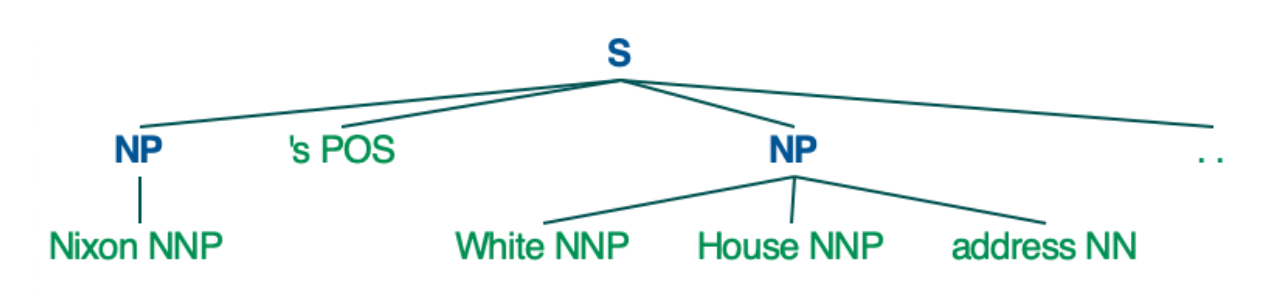
\includegraphics[width=0.70\textwidth]{Figures/tree.png}
          \caption{nltk tree formed from grammar by RegexParser.}
           \label{tree}
\end{figure}

The extracted nouns, represented by the “NP” label, in this example would be “Nixon” and “White House address”.

Named entities are also extracted from the text; this is done using the ne\_chunk() method in the nltk.chunk package. A named entity is considered to be names of people, locations, organizations, products, etc. Given the same input the ne\_chunk() method produces the following tree.
\begin{figure}[h]
    \centering
         
\includegraphics[width=0.70\textwidth]{Figures/treeNE.png}
          \caption{nltk tree formed from ne\_chunk().}
           \label{treeNE}
\end{figure}

Similarly named entities are those with a “NE” label, thus the named entities extracted are “Nixon” and “White House”. 

Both the named entities and the noun pairs are further processed to be all lowercase. The final set of concepts is the union between the list of found noun pairs and named entities. Concepts that are extracted from the example sentence are therefore [“nixon”, “white house address”, “white house”]. 

\subsection{Model Generation}
The Corpus.concepts object provides a bag-of-concepts representation. Corpus.concepts is a list that contains a list of concepts for each document. This representation and its benefits are discussed in Section \ref{subsec:3.5.1}. LDA uses this representation to construct a topic model from the corpus of documents. The construction of the corpus topic model is done by using the Model class in Model.py. The Model class uses the python package gensim \citep{rehurek2010software} to create a LDA model from the bag-of-concepts representation in Corpus.concepts. First a dictionary from the bag-of-concepts is created using the gensim.corpora Dictionary class. A dictionary is an object that maps each unique concept to a unique id. The Model class then uses this dictionary to produce a processed bag-of-concepts representation which contains a list that contains a list for each document. The list of a document contains tuples of concept id’s (from the dictionary) and their frequency in the document, see the following for a simple example.

\begin{itemize}
    \item \textbf{Bag-of-concepts}: [[“nixon”, “watergate”, “nixon”], [“impeachment”, “nixon”, “president ford”]]
    \item \textbf{Dictionary}: [(0,“nixon”),(1,”watergate”),(2,“impeachment”),(3,“president ford”)]
    \item \textbf{Processed bag-of-concepts}: [[(0,2), (1,1)], [(2,1), (0,1), (3,1)]]
\end{itemize}

Using the dictionary and the processed bag-of-concepts representation a model is formed using gensim.model.LdaModel(). The LdaModel uses a series of parameters to create a topic model, shown in Figure \ref{topicModel} provided from the python package pyLDAvis \citep{sievert2014ldavis}. The parameters used in the formation of the model are as follows:
\begin{itemize}
    \item \textbf{Corpus} – which is passed the processed bag-of-concepts object.
    \item \textbf{Id2word} – which is passed the dictionary object.
    \item \textbf{num\_topics} – passed the number of topics for model creation specified in the parameters of the Model class.
    \item \textbf{random\_state} – passed a static value of 100 which is used in the creation of the random priori using in model creation, this is static for model reproducibility.
    \item \textbf{update\_every} – passed a static value of 1. This specifies that parameters of the statistical model should be updated from every document passed into it.
    \item \textbf{passes} – passed a static value of 3, the number of passes over the corpus set of document
    \item \textbf{alpha} – set to auto, the alpha value is the priori belief for each topics’ probability, when set to auto the model learns an asymmetric prior from the corpus.
\end{itemize}

The crucial parameters for lda are the k number of topics latent topics and the hyper parameters such as alpha which describe the priori probability distribution between topics. There has been much work done to attempt to determine how to best select these parameters \citep{yau2014clustering,carter2016reading}, but there are no conclusive ways to determine the most optimal parameters when LDA is used in a wider system because certain model results from use of different parameters have different effects when LDA is used in larger system. Thus practical testing is the best way to determine these parameters \citep{suominen2016map}. The parameters here were assessed in an attempt to produce adequate models to be used in the summarisation system, but further evaluation could be performed to determine the optimal values for parameters with the effect of improving the personalised retrieval performance in the system.

\begin{figure}[h]
    \centering
         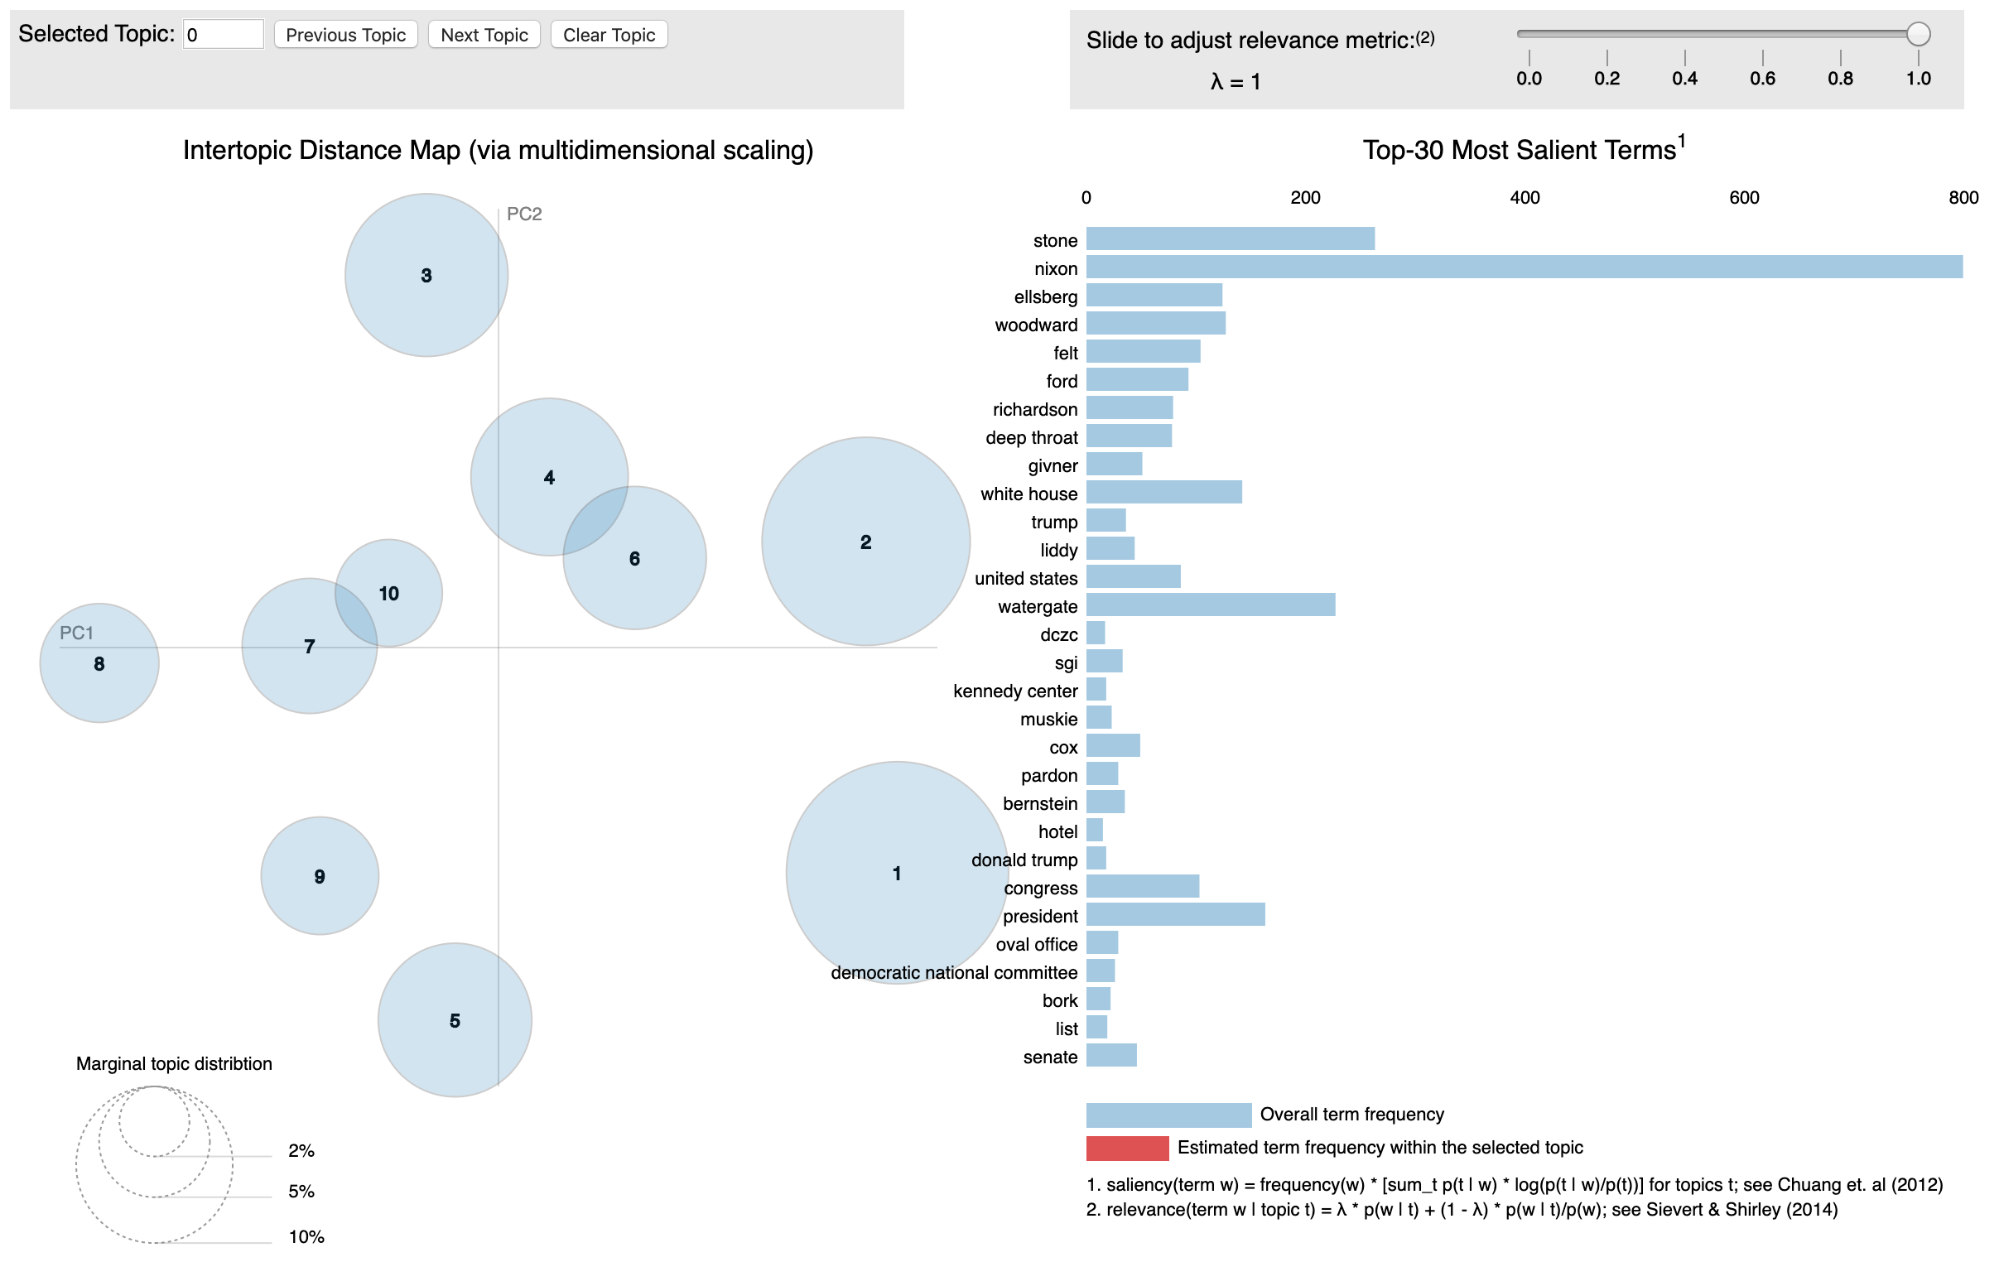
\includegraphics[width=1.0\textwidth]{Figures/ldamodel.png}
          \caption{pyLDAvis visualisation of topic model formed from Watergate Scandal Wikipedia articles.}
           \label{topicModel}
\end{figure}

\subsection{Summary of Model and Corpus Generation}
This series of processes work together to take the raw XML dumps of Wikipedia articles and create both Corpus object and Model object to be used in other parts of the summarisation system. The Corpus object parses articles into a series of Documents. Each Document object uses the Concepts class to create three structures: a dictionary modeling a mapping from sentences to concepts, a dictionary modeling a mapping from concepts to sentences, and a list of concepts found in the document. Each structure formed in a document gets added to the corresponding structures in the Corpus class, creating the same structures for all sentences and concepts in the input documents. The three data structures in the Corpus object will be used in all other aspects of the system to provide a variety of tasks for summarisation. The Model object creates and contains a LDA topic model, generated from the bag-of-concepts presentation in Corpus.concepts. This topic model will be used in retrieval of documents. The processes outlined in this section are the foundation for the rest of the processes performed in the summarisation system.

\section{Query-Based Document Retrieval}
The query-based document retrieval process of the system allows for the retrieval of a subset of the corpus set based on a specified query. A query relevant document set is passed into the summarisation process of the system, in order to provide a query based summarisation. This process of the system has two processes: query expansion and query document retrieval. The Query class, defined in Query.py, handles both the expansion of queries via cross concept chains as well as the retrieval of relevant documents in the corpus. Queries for this system are expressed using a sub set of concepts that are contained in the extracted set of document concepts. They are expanded from selecting all sentences containing the concepts given in the query to create a new document.  A specified number of additional relevant terms are selected based on the topic distribution of the new document. The expanded query is then used to determine a set of documents that are relevant based on the similarity of a query topic distribution and individual document’s topic distribution from the corpus. Documents with a similarity above a threshold are added to a list of documents to summarise in the summary generation process of the system.  These two processes and their implementation are discussed in this section.

\subsection{Query Expansion}
As discussed in Section \ref{subsec:3.5.3}, query expansion is a technique used to improve retrieval of documents. The output of expansion in this system are cross concepts chain queries done using the method presented by Li and Jin’s \citeyear{li2016cross} paper “Cross-document knowledge discovery using semantic concept topic model.” In \emph{2016 15th IEEE International Conference on Machine Learning and Applications (ICMLA)}. A query will contain a set of concepts that each relate to a various number of latent topics in the topic model. The aim is to add supplemental concepts to bolster the topic distribution in the original query, or to represent concepts from a hidden topic that connects topics discussed in the original query. This process uses a set of steps to produce a new expanded query topic distribution for query-based document retrieval. This implementation follows closely Li and Jin’s \citeyear{li2016cross} cross concept chain method.

\begin{figure}[h]
    \centering
         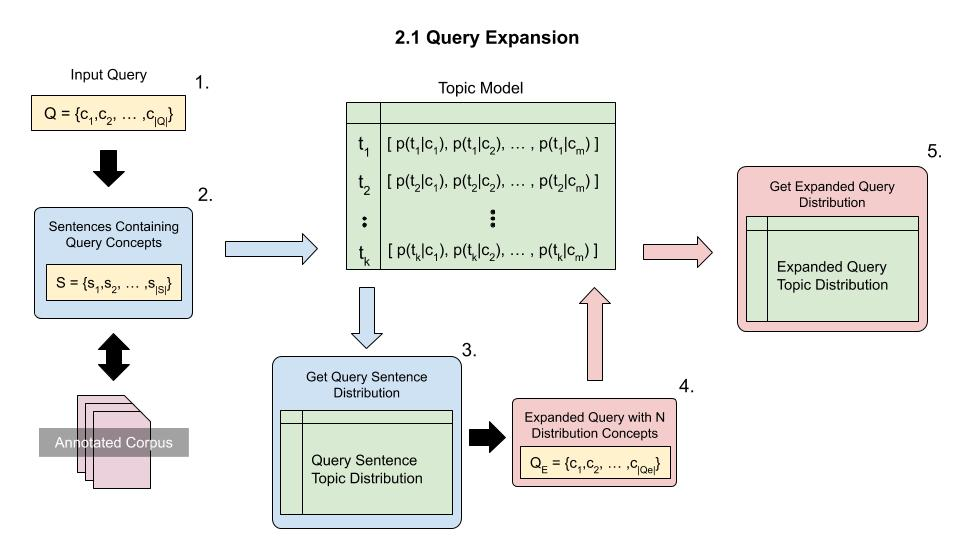
\includegraphics[width=1.0\textwidth]{Figures/System_Design_Query-Based_Retrieval.jpg}
          \caption{Process of expanding a query}
           \label{queryExp}
\end{figure}
Where $Q$ is the set of concepts that describe a query. $S$ is the set of sentences retrieved from the corpus that contains concepts given in $Q$. $Q_E$ is the union of the set of most relevant concepts extracted from the topic distribution of $S$ and the concepts from the original concept set $Q$.

Query expansion is done via the Query class defined in Query.py. A Query object is created by specifying a Corpus and Model object. These objects are created in the Corpus and Model generation process of the system. The expansion of an input query is done as the first step in the retrieve\_docs() method from a Query object. Expansion of queries is done via the get\_concept\_chain() method which uses the following parameters:

\begin{itemize}
    \item \textbf{concepts} – a query expressed as a list of concepts.
    \item \textbf{keywords} – a number specifying the final size of the expanded query.
\end{itemize}

This method follows the steps of the query expansion processes shown in Figure \ref{queryExp}. Step 2 in the processes uses the Corpus.con2sen object to find sentences that contain each of the concepts that are inputted in Step 1. The sentences are joined together to form a new document. This document is used in creating a new Model object in Step 3, producing a document specific lda model. Each topic found by this new lda model is iterated over in Step 4. For each of the topic\_ids in the new model are passed into the gensim.ldamodel method get\_topic\_terms(). This method takes topic\_id and number of terms and produces the top number of terms and their probabilities relating to a given topic\_id. The probability of the term relating to a query is given by  multiplying  the topic\_id probability and the probability of term relating to the topic\_id. Each of these top terms and their found probability are added into a list top\_n\_words. The top\_n\_words list is sorted and then iterated over. Words from the top\_n\_words lists are added to a list called cross\_chain\_query if they are not contained in the original query and the cross\_chain\_query length is less than the specified expanded length in the keywords parameter. The original query and  the new found words are combined to produce a cross concept chain expanded query. Step 5 uses this new query and passes it into the Model.lda\_model to get a topic distribution. This topic distribution is used in finding similar documents in the following query-based retrieval processes.

\subsection{Query-Based Document Retrieval}
This process takes an expanded query topic distribution and produces a subset of the corpus documents that are relevant to a query based examining the similarity of each document's topic distribution with the given query topic distribution. The topic distribution of any given document or query is a vector of latent topic\_ids and their corresponding probabilities of relating to the input. These vectors can be compared using a cosine similarity metric. The resulting documents can then be selected to be relevant based on a set threshold of similarity. This process is done in the Query class method retrieve\_docs():

\begin{lstlisting}[language=Python]
def retrieve_docs(self, concepts: [str], similarity = 0.80, query_len=10):
    # topic_dist = self.model.topic_dist(concepts)
    topic_dist = self.get_concept_chain(concepts, keywords=query_len)
    similar_docs = []
    count = 0
    for doc in self.corpus.docs:
        for sent in doc.sen2con.keys():
            sent_concepts = doc.sen2con[sent]
            doc_dist = self.model.topic_dist(sent_concepts)
            sim = cossim(doc_dist[0], topic_dist[0])
            if sim > similarity:
                count+=1
                similar_docs.append(sent)
    
    return similar_docs, topic_dist
\end{lstlisting}
retrieve\_docs() first expands a query using the method get\_concept\_chain(). The get\_concept\_chain() returns a topic distribution of an expanded query. For each Document in the Corpus object doc list, the concepts of the Document are passed into the Model objects topic\_dist method(). The similarity of the topic distribution of a Document and the expanded query is determined from using the gensim.matutils method cossim(). If the similarity is greater than the similarity threshold, the Document object text is added to a list that is returned at the end of execution. The returned list of document text is what is used in the summary generation process of the system discussed in the next section.

\section{Summary Generation}
The summary generation process of the system takes a set of relevant documents produced from the query-based document retrieval process and produces a summary. The summary process produces a summary via two processes: sentence scoring and summary generation. The implementations for both these processes are based on the method presented by Alguliev et al. \citeyear{alguliev2011mcmr} “MCMR: Maximum coverage and minimum redundant text summarization model” in \emph{Expert Systems with Applications}. Further discussion of this method is presented in Section \ref{subsec:3.5.4}. This method of summarisation treats summary formation as an optimisation problem, where the scores of combinations of sentences are combined in an attempt to maximise a summary score under the constraint of length. The matematical form of this problem is given in (\ref{mcmrFull}). Alguliev et al. approach is implemented within the Summary class in Summary.py. The Summary class takes in four parameters:

\begin{itemize}
    \item \textbf{doc} – a list of sentences that are considered for summarisation.
    \item \textbf{corpus} – a Corpus object created on all documents.
    \item \textbf{min\_len} – the minimum sentence length, in characters, to be considered for a summary.
    \item \textbf{num\_processes} – the number of python process used for sentence scoring.
\end{itemize}

\subsection{Sentence Scoring}
The Summary class calculates all considered combinations of sentences when initialised. This sentence scoring is done upon initialization to allow the scoring of combinations of sentences to be done concurrently. Before individual sentences are scored the list of sentences considered is pruned.

Sentences are removed from the list if they are: shorter than the length threshold specified in the min\_len parameter, redundant (the same sentence exists somewhere else in the list), or if the set of concepts extracted from the sentence is empty (accessed from Corpus.sen2con[sentence]). The pruned sentence list is then set to the Summary.sentences object (i.e self.sentences = pruned\_sentences). After the input sentences have been preprocessed the Summary class forms 3 data structures to be used in sentence scoring:

\begin{itemize}
    \item \textbf{self.sen\_con\_freq} – a python dictionary which uses each concept in the sentences list as key and a list of sentences that contain that concept as a value.
    \item \textbf{self.con\_freq} – a python dictionary which uses each concept in the sentences list as key a number occurrences of that concept in the set of sentences as a value.
    \item \textbf{term\_sent\_weights} – a dictionary of dictionaries where the parent dictionary uses each sentence as a key with a child dictionary as a value dictionary. The child dictionary uses concepts in a sentence as keys and the value is that terms tf-isf score calculated via (\ref{tfisf})
\end{itemize}

These structures are created in the method self.\_\_sent\_term\_weighting() in the Summary class. Once these structures are created a list of pairs of sentences is constructed and scored. This list of sentence pairs to be scored is created by the following for loop which is based on the double summation given from the mathematical formalisation:

\begin{lstlisting}[language=Python]
sentences_pairs = []
for i in range(0, len(sentences)-2):
    for j in range(i+1, len(sentences)-1):
        sentences_pairs.append((sentences[i], sentences[j]))
\end{lstlisting}

For each sentence pair the two scores for the respective pair are calculated using the generalised form of a similarity score, used in (\ref{mcmrGeneral}):
\begin{equation}
    score(s_i,s_j) = sim(D,s_i) + sim(D,s_j) - sim(s_i,s_j)
    \label{generalised}
\end{equation}

The similarity was calculated using two metrics: the cosine similarity and Normalised Google Distance (NGD). For each pair a score was calculated and stored in a dictionary.

The cosine similarity was calculated using the term\_sent\_weights object that was previously constructed. The three cosine similarity scores from (\ref{generalised}) were calculated using the cos\_sim function:

\begin{lstlisting}[language=Python]
def cos_sim(self, item1, term_sent_weights, con_freq, item2=None):
    item2_vec = []
    item1_vec = list((term_sent_weights[item1]).values())
    if item2 is None:
        item2_vec = list(con_freq.values())
    else:
        item2_vec = list((term_sent_weights[item2]).values())
    numerator = dot(item1_vec, item2_vec)
    denominator = (norm(item1_vec)*norm(item2_vec))
    similarity = numerator/denominator
    return similarity
\end{lstlisting}

Each sentence or document is first represented as a list by all the term weights for all the concepts that are contained within them. The cosine similarity is calculated from the dot product of the concept weights over the multiplication of the two vectors normalisation.

The normalised google distance for a sentence pair was calculated for three scores of the generalised similarity score formula (\ref{generalised}). The ngd score was calculated by ngd\_sim and ngd\_term method based on (\ref{ngdSent}) and (\ref{ngdTerm}) respectively:

\begin{lstlisting}[language=Python]
def ngd_sim(self, item1, n, sent_con_freq, con2sen, item2=None,):
    item2_con = []
    item1_con = con2sen[item1]
    if item2 is None:
       item2_con = list(sent_con_freq.keys())
    else:
       item2_con = con2sen[item2]
    ngd_sum = 0
    ngds_counted = 0
    for term1 in item1_con:
        for term2 in item2_con:
            ngds_counted += 1
            ngd = self.ngd_term(term1, term2, n, sent_con_freq)
            ngd_sim = math.exp(-ngd)
            ngd_sum += ngd_sim
   ngd = (ngd_sum/(len(item1_con) * len(item2_con)))
   return ngd

def ngd_term(self, t1, t2, n, sent_con_freq):
    t1_sen_count = len(sent_con_freq[t1])
    t2_sen_count = len(sent_con_freq[t2])
    t1_t2_sen_count = len([con for con in sent_con_freq[t1] if con in sent_con_freq[t2]])
    t1_log = math.log10(t1_sen_count)
    t2_log = math.log10(t2_sen_count)
    t1_t2_log = 0
    if(t1_t2_sen_count > 0):
        t1_t2_log = math.log10(t1_t2_sen_count)
    numerator = max(t1_log,t2_log) - t1_t2_log
    denominator = math.log10(n) - min(t1_log, t2_log)
    return (numerator/denominator)
\end{lstlisting}

From precalculating the scores of the sentence pairs in this implementation, the original maximization functions (\ref{mcmrFull}) is simplified to the following:

\begin{equation}
    Maximize \; f_{\alpha} = \sum_{i=1}^{n-1} \sum_{j=i+1}^n [\alpha(score_{cos}(s_i,s_j)) + (1-\alpha)(score_{ngd}(s_i,s_j))]x_{ij}
    \label{myMcmr}
\end{equation}

Inorder to reduce the time to generate a summary the scoring of sentence pairs is done concurrently. The list of sentence pairs is spit up evenly between a specified number of processes. These processes construct two dictionaries: one that contains the cosine similarity and one that contains the NGD scores of the senect pairs, where each sentence pair is a key to the respective score.

\subsection{Summary Formation}
The approach to the summary formation, the simplified maximisation function (15), given from precalculating the scores, must be formulated as an integer linear programming problem. The aim is to adjust the binary $x_{ij}$ variables to produce the highest scoring summary possible from the set of sentences. The resulting values of the $x_{ij}$ will identify the sentence pairs that should be contained in the final summary. The python package PuLP \citep{mitchell2011pulp} was used to implement (\ref{myMcmr}) as linear programming problem in the doc\_summary method:

\begin{lstlisting}[language=Python]
def doc_summary(self, sen_len=300, alpha=0.8):
    sentences = self.doc
    n_i = len(sentences) - 2
    n_j = len(sentences) - 1
    maxium_len = sen_len
    lp_problem = p.LpProblem('problem', p.LpMaximize)
    x_ij = p.LpVariable.dicts('xij', [(sentences[i],sentences[j]) for i in range(0, n_i) for j in range(i+1, n_j)], cat='Binary')
    constriant_len = p.LpConstraint(e=p.lpSum([(len(sentences[i]) + len(sentences[j]))*(x_ij[(sentences[i],sentences[j])]) for i in range(0, n_i) for j in range(i+1, n_j)]),sense=p.LpConstraintLE,rhs=300)

    objective = p.lpSum([ \
        (alpha * (self.find_cos_sim(i, j, sentences) * x_ij[(sentences[i],sentences[j])])) \
        + \
        ((1-alpha) * (self.find_ngd_sim(i, j, sentences) * x_ij[(sentences[i],sentences[j])]))
            for i in range(0, len(sentences)-2) for j in range(i+1, len(sentences)-1)])
    lp_problem += objective
    lp_problem += constriant_len

    maxium_summary_sent = []
    lp_problem.solve()

    summary_sent = {}
    variables_dict = {}
    variables_list = lp_problem.variables()
    for v in variables_list:
        variables_dict[v.name] = v.varValue
    variables_keys = list(variables_dict.keys())

    index = 0
    for i in range(0, len(sentences)-2):
        for j in range(i+1, len(sentences)-1):
            key = variables_keys[index]

            if variables_dict[key] > 0:
                summary_sent[sentences[i]] = ""
                summary_sent[sentences[j]] = ""
            index+=1

    return list(summary_sent.keys())
\end{lstlisting}

First a pulp LpProblem was initialised to maximise. Then a set of binary LpVariables was constructed representing pairs of sentences to be included in the summary. The length constraint was then added to the LpProblem specifying that the length of all sentence pairs to be included in the summary should be no longer than the specified sentence length. Then the objective was expressed in the same form as (\ref{myMcmr}) using the precalculated cosine and NGD similarity for sentence pair variables. Then the problem is solved by PuLP. The result is binary values of variables that represent sentence pairs to be included in the summary. These set of variables are iterated over to extract the set of sentences which should be included in the summary. The result is a list of sentences that the summary problem is maximised from.

\section{Summary}
The implementation of the processes of the system design have been described in this chapter. From the python classes the processes can be linked together to provide the functionality of the summarisation system. A simple example of how these classes are used is the following:

\begin{lstlisting}[language=Python]
corpus = Corpus([], filename='./WikiCorpus/WaterGateText/AA/wiki_00', regen=False)
concepts = corpus.get_concepts()
model = Model(concepts),topics=10)
query = Query(corpus, model)
Query_concepts = ["operation sandwedge", "political enemies", "caulfield"]
found_docs, query_topic_dist = query.retrieve_docs(query_concepts, similarity=0.80, query_len=20)
summary = Summary(found_docs, corpus)
summary_list = summary.doc_summary()
links = []
    for sent in summary_list:
        title, link = corpus.get_links(sent)
        if (title, link) not in links:
            links.append((title, link)) 
\end{lstlisting}

Implementing these methods into classes allows for a great deal of flexibility in constructing the methods to perform summarisation. From methods encapsulation they can individually be tested for correctness of implementation. The modularity of a class based implementation also allows for the parts of the system to be tested as single processes of the whole. The result is an implementation that produces the functionality outlined by the design that can be used to assess the system’s design extent of performing domain specific personalised summarisation without the use of formal ontologies.

\chapter{Evaluation}
\section{Introduction}
Inorder to address the extent to which the proposed domain independent summarisation system can perform extractive personalised summarisation, two forms of evaluation were performed, referred to as Analysis 1 and 2. 

Analysis 1 set out to determine the efficacy of the systems summarisation method, the system was tested on two summarisation data sets, a single document and multi-document dataset. From the summaries produced ROUGE metrics (Lin, Cao, Gao, and Nie, 2006) were calculated and compared to other extractive summarisation systems. The aim of the comparative evaluation was to determine both the quality of summaries produced against human generated summaries as well as the systems performance against state of the art extractive summarisation systems. 

Analysis 2 examines the systems ability to provide personalised summarisation, through the use of queries. Two types of queries were examined, a context free query and contextual query. Context free queries examine the system's ability to retrieve relevant documents and produce a human interpretable summary within a specific domain. The second type of query was to assess the efficacy of the system to be used in a recommender system from examining system summaries produced from a context and context free query in specific domains. The results of comparative evaluation show that the system does achieve state of the art summarisation performance, but is a competitive method for summarisation. The results of query based summarisation evaluation, demonstrate the system's effectiveness to be providing personalised summaries in a specific domain, and the possible use of the summarisation system in a recommender system.

\section{Analysis 1: Comparative Summarisation Evaluation}
The comparative evaluation of this system with state of the art are extractive summarisation systems assess the implementation of existing methods in the system to perform generic summarisation. The metrics to use in the comparative evaluation are the ROUGE (Recall-Oriented Understudy for Gisting Evaluation) metrics \citep{lin2004rouge}. ROUGE metrics are used for evaluating how well automatic summarisation methods can produce summaries similar to a human generated reference summary. The ROUGE metrics used are:

\begin{itemize}
    \item ROUGE-1: The overlap of uni-grams (single terms) between a system summary and a reference summary.
    \item ROUGE-2: The overlap of bi-grams (adjacent terms) between a system summary and a reference summary. This is provide by the following formula:
\end{itemize}

Each ROUGE metric uses two methods of scoring, precision and recall. Recall accounts for how well the system summary is able to cover the content of the reference summary. The precision of a summary asses how much of the system summary is relevant to the reverence summary. These two calculations can be generalised as the following equations:

\begin{equation*}
    ROUGE_{recall} = \frac{\#\:of\: Overlaps\: of \:System\: Content \:and \:Reference\: Content}{\#\: of\: Content\: in\: Reference\: Summary}
    \label{rouge_r2}
\end{equation*}

\begin{equation*}
    ROUGE_{precision} = \frac{\# \:of\: Overlaps\: of\: System\: Content\: and\: Reference\: Content}{\#\: of\: Content\: in\: System\: Summary}
    \label{rouge_p3}
\end{equation*}
\chapter{Conclusion}
\bibliographystyle{agsm}
\bibliography{bibs/sample}
\setcitestyle{semicolon}
\appendix
\renewcommand{\thechapter}{A\arabic{chapter}}


\end{document}